\documentclass{tufte-handout}
\title{Diagonalization, SVD \& The Power Method \thanks{Author: Wayne Small}}
\usepackage{amsmath}  % extended mathematics
\usepackage{amstext}
\usepackage{amssymb}
\usepackage{amsthm}
\usepackage{amsfonts}
\usepackage{mathtools}
\usepackage{multirow}
\renewcommand{\familydefault}{\sfdefault}
\geometry{left=0.25in, right=2.6in}
\usepackage{tikz}
\newcommand*\circled[1]{\tikz[baseline=(char.base)]{
		\node[shape=circle,draw,inner sep=2pt] (char) {#1};}}
\newcommand{\norm}[1]{\left\lVert#1\right\rVert}
\renewcommand{\qedsymbol}{$\blacksquare$}
\newcommand{\Waynehref}[3][blue]{\href{#2}{\color{#1}{#3}}}%

\begin{document}

\[\]
{\Large\textbf{Definition 1: Eigendecomposition \& Diagonalization}}\\\leavevmode\\
\noindent Suppose an n by n matrix $A$ has n linearly independent eigenvectors $\mathbf{x}_1$, $\mathbf{x}_2$, ..., $\mathbf{x}_n$. Put them into the columns of the \textbf{eigenvector matrix} $\mathbf{X}$. Then $\mathbf{\Lambda}\equiv\mathbf{X}^{-1}\mathbf{A}\mathbf{X}$ is the \textbf{eigenvalue matrix}. $A$ has been \textbf{diagonalized}.
\[
\mathbf{\Lambda}\equiv\mathbf{X}^{-1}\mathbf{A}\mathbf{X}
~~~~~~~~~~~~
\mathbf{A}\mathbf{X}= \mathbf{X}\mathbf{\Lambda}
~~~~~~~~~~~~
\mathbf{A}= \mathbf{X}\mathbf{\Lambda}\mathbf{X}^{-1}
\]\\\leavevmode\\
\noindent $\mathbf{X}\mathbf{\Lambda}\mathbf{X}^{-1}$ is called the \textbf{eigendecomposition} of $A$. But what does the eigenvalue matrix $\mathbf{\Lambda}$ look like? Why do we say $A$ has been "diagonalized"?\\\leavevmode

\noindent{\Large\textbf{Lemma 1: Eigenvalue Matrix Is Diagonal With Eigenvalues In Diagonal}}\\\leavevmode\\
\noindent Suppose an n by n matrix $A$ has n linearly independent eigenvectors $\mathbf{x}_1$, $\mathbf{x}_2$, ..., $\mathbf{x}_n$. Then the eigenvalue matrix $\mathbf{\Lambda}\equiv\mathbf{X}^{-1}\mathbf{A}\mathbf{X}$ is a diagonal matrix with the eigenvalues in the diagonal.\\\leavevmode\\
\noindent\textbf{Proof:}\\
\noindent $AX$ and $X\Lambda$ are both equal to $\begin{bmatrix*}[c]
\lambda_1\mathbf{x}_1&\dots&\lambda_n\mathbf{x}_n
\end{bmatrix*}$:
\[
AX=
\begin{bmatrix*}[c]
\mathbf{a}_1\\ \vdots \\ \mathbf{a}_n
\end{bmatrix*}
\begin{bmatrix*}[c]
\mathbf{x}_1&\dots&\mathbf{x}_n
\end{bmatrix*}
=
\begin{bmatrix*}[c]
\mathbf{a}_1\mathbf{x}_1&\mathbf{a}_1\mathbf{x}_2&\dots&\mathbf{a}_1\mathbf{x}_n\\
\mathbf{a}_2\mathbf{x}_1&\mathbf{a}_2\mathbf{x}_2&\dots&\mathbf{a}_2\mathbf{x}_n\\
\vdots&\vdots&\ddots&\vdots\\
\mathbf{a}_n\mathbf{x}_1&\mathbf{a}_n\mathbf{x}_2&\dots&\mathbf{a}_n\mathbf{x}_n
\end{bmatrix*}
\]
\[
=
\begin{bmatrix*}[c]
A\mathbf{x}_1&\dots&A\mathbf{x}_n
\end{bmatrix*}
=
\begin{bmatrix*}[c]
\lambda_1\mathbf{x}_1&\dots&\lambda_n\mathbf{x}_n
\end{bmatrix*}
\]
\[
X\Lambda=
\begin{bmatrix*}[c]
\mathbf{x}_1&\dots&\mathbf{x}_n
\end{bmatrix*}
\begin{bmatrix*}[c]
\lambda_1&&&\\
&\lambda_2&&\\
&&\ddots&\\
&&&\lambda_n
\end{bmatrix*}
=
\begin{bmatrix*}[c]
x_{1,1}&x_{2,1}&\dots&x_{n,1}\\
x_{1,2}&x_{2,2}&\dots&x_{n,2}\\
\vdots&\vdots&\ddots&\vdots\\
x_{1,n}&x_{2,n}&\dots&x_{n,n}
\end{bmatrix*}
\begin{bmatrix*}[c]
\lambda_1&&&\\
&\lambda_2&&\\
&&\ddots&\\
&&&\lambda_n
\end{bmatrix*}
\]
\[
=
\begin{bmatrix*}[c]
x_{1,1}\lambda_1&x_{2,1}\lambda_2&\dots&x_{n,1}\lambda_n\\
x_{1,2}\lambda_1&x_{2,2}\lambda_2&\dots&x_{n,2}\lambda_n\\
\vdots&\vdots&\ddots&\vdots\\
x_{1,n}\lambda_1&x_{2,n}\lambda_2&\dots&x_{n,n}\lambda_n
\end{bmatrix*}
=
\begin{bmatrix*}[c]
\lambda_1\mathbf{x}_1&\dots&\lambda_n\mathbf{x}_n
\end{bmatrix*}
\]
The eigenvectors are linearly independent, so $X$ is invertible and we have
\[
\mathbf{X}^{-1}\mathbf{A}\mathbf{X}= \mathbf{\Lambda}
~~~~~~~~~~~~
\mathbf{A}\mathbf{X}= \mathbf{X}\mathbf{\Lambda}
~~~~~~~~~~~~
\mathbf{A}= \mathbf{X}\mathbf{\Lambda}\mathbf{X}^{-1}
\]
\noindent\qedsymbol\\\leavevmode\\
\noindent Let's try an example:\\\leavevmode
\[
A=
\begin{bmatrix*}[c] 1&2\\4&3 \end{bmatrix*}
\rightarrow
0=
\begin{vmatrix*}[c] 1-\lambda&2\\4&3-\lambda \end{vmatrix*}
=(1-\lambda)(3-\lambda)-8
=\lambda^2-4\lambda+3-8
\]
\[
=\lambda^2-4\lambda-5
=(\lambda+1)(\lambda-5)
\implies
\lambda_1=-1
~~~~~
\lambda_2=5
\]
\[
\text{Let's check:}~~
\vert A\vert=1\cdot3-2\cdot4=-5=\lambda_1\cdot\lambda_2
~~~~~~~
tr(A)=4=\lambda_1+\lambda_2
\]
\[
\lambda_1=-1
\rightarrow
\begin{bmatrix*}[c] 1-\lambda_1&2\\4&3-\lambda_1 \end{bmatrix*}
=
\begin{bmatrix*}[c] 2&2\\4&4 \end{bmatrix*}
\rightarrow
\begin{bmatrix*}[c] 1&1\\0&0 \end{bmatrix*}
\rightarrow
\mathbf{x_1}=
\begin{bmatrix*}[c] -1\\1 \end{bmatrix*}
\]
\[
A\mathbf{x_1}=
\begin{bmatrix*}[c] 1&2\\4&3 \end{bmatrix*}
\begin{bmatrix*}[c] -1\\1 \end{bmatrix*}
=
\begin{bmatrix*}[c] -1+2\\-4+3 \end{bmatrix*}
=
\begin{bmatrix*}[c] 1\\-1 \end{bmatrix*}
=\lambda_1\mathbf{x_1}
\]
\[
\lambda_2=5
\rightarrow
\begin{bmatrix*}[c] 1-\lambda_2&2\\4&3-\lambda_2 \end{bmatrix*}
=
\begin{bmatrix*}[c] -4&2\\4&-2 \end{bmatrix*}
\rightarrow
\begin{bmatrix*}[c] 1&-\frac{1}{2}\\0&0 \end{bmatrix*}
\rightarrow
\mathbf{x_2}=
\begin{bmatrix*}[c] \frac{1}{2}\\1 \end{bmatrix*}
\]
\[
A\mathbf{x_2}=
\begin{bmatrix*}[c] 1&2\\4&3 \end{bmatrix*}
\begin{bmatrix*}[c] \frac{1}{2}\\1 \end{bmatrix*}
=
\begin{bmatrix*}[c] \frac{1}{2}+2\\2+3 \end{bmatrix*}
=
\begin{bmatrix*}[c] 2\frac{1}{2}\\5 \end{bmatrix*}
=\lambda_2\mathbf{x_2}
\]
Let's check that our eigenvectors are independent:
\[
\begin{bmatrix*}[c] 0\\0 \end{bmatrix*}
=
\begin{bmatrix*}[c] -1&\frac{1}{2}\\1&1 \end{bmatrix*}
\begin{bmatrix*}[c] c_1\\c_2 \end{bmatrix*}
\]
\[
\begin{bmatrix*}[c] -1&\frac{1}{2}\\1&1 \end{bmatrix*}
\rightarrow
\begin{bmatrix*}[c] -1&\frac{1}{2}\\0&\frac{3}{2} \end{bmatrix*}
\rightarrow
\begin{bmatrix*}[c] -1&0\\0&1 \end{bmatrix*}
\rightarrow
\begin{bmatrix*}[c] 1&0\\0&1 \end{bmatrix*}
\]
\[
\implies
\text{No free variables and nullspace $=$ \{$\mathbf{0}$\}}
\]
And let's calculate $X^{-1}$:
\[
X^{-1}=\frac{1}{\vert X\vert}adj(X)=
\frac{1}{-1-\frac{1}{2}}
\begin{bmatrix*}[c] 1&-\frac{1}{2}\\-1&-1 \end{bmatrix*}
=
-\frac{2}{3}
\begin{bmatrix*}[c] 1&-\frac{1}{2}\\-1&-1 \end{bmatrix*}
\]
And check the inverse calculation:
\[
X^{-1}X=
-\frac{2}{3}
\begin{bmatrix*}[c] 1&-\frac{1}{2}\\-1&-1 \end{bmatrix*}
\begin{bmatrix*}[c] -1&\frac{1}{2}\\1&1 \end{bmatrix*}
=
-\frac{2}{3}
\begin{bmatrix*}[c] -1-\frac{1}{2}&\frac{1}{2}-\frac{1}{2}\\1-1&-\frac{1}{2}-1 \end{bmatrix*}
=
-\frac{2}{3}
\begin{bmatrix*}[c] -\frac{3}{2}&0\\0&-\frac{3}{2} \end{bmatrix*}
=I
\]
And, finally, let's diagonlize $A$:
\[
X\Lambda X^{-1}=
\begin{bmatrix*}[c] -1&\frac{1}{2}\\1&1 \end{bmatrix*}
\begin{bmatrix*}[c] \lambda_1&0\\0&\lambda_2 \end{bmatrix*}
\Big(-\frac{2}{3}\Big)
\begin{bmatrix*}[c] 1&-\frac{1}{2}\\-1&-1 \end{bmatrix*}
\]
\[
=
\Big(-\frac{2}{3}\Big)
\begin{bmatrix*}[c] -1&\frac{1}{2}\\1&1 \end{bmatrix*}
\begin{bmatrix*}[c] -1&0\\0&5 \end{bmatrix*}
\begin{bmatrix*}[c] 1&-\frac{1}{2}\\-1&-1 \end{bmatrix*}
\]
\[
=
\Big(-\frac{2}{3}\Big)
\begin{bmatrix*}[c] -1&\frac{1}{2}\\1&1 \end{bmatrix*}
\begin{bmatrix*}[c] -1&\frac{1}{2}\\-5&-5 \end{bmatrix*}
=
\Big(-\frac{2}{3}\Big)
\begin{bmatrix*}[c] 1-\frac{5}{2}&-\frac{1}{2}-\frac{5}{2}\\-1-5&\frac{1}{2}-5 \end{bmatrix*}
\]
\[
=
\Big(-\frac{2}{3}\Big)
\begin{bmatrix*}[c] -\frac{3}{2}&-\frac{6}{2}\\-6&-\frac{9}{2} \end{bmatrix*}
=
\frac{2}{3}
\begin{bmatrix*}[c] \frac{3}{2}&\frac{6}{2}\\6&\frac{9}{2} \end{bmatrix*}
=A
\]
\[\]
\noindent So we can't just diagonalize any ol' square matrix? How do we know which matrices have independent eigenvectors? Please don't tell me that we have to compute the eigenvectors to see if they're independent.\\\leavevmode

\noindent{\Large\textbf{Lemma 2: Independent Eigenvectors From Distinct Eigenvalues}}\\\leavevmode\\
\noindent The eigenvectors from distinct eigenvalues are linearly independent.\\\leavevmode\\
\noindent\textbf{Proof:}\\
\noindent Suppose $\sum_{i=1}^{n}c_i\mathbf{x_i}=\mathbf{0}$. Multiply by $A$ and $\lambda_n$ to get two equations:
\[
\mathbf{0}=A\sum_{i=1}^{n}c_i\mathbf{x}_i
=\sum_{i=1}^{n}c_iA\mathbf{x}_i
=\sum_{i=1}^{n}c_i\lambda_i\mathbf{x}_i
\]
\[
\mathbf{0}=\lambda_n\sum_{i=1}^{n}c_i\mathbf{x}_i
=\sum_{i=1}^{n}c_i\lambda_n\mathbf{x}_i
\]
Subtract those two equations so that the coefficient of $\mathbf{x}_n$ is $\lambda_n-\lambda_n$ and $\mathbf{x}_n$ is gone. Now multiply by $A$ and $\lambda_{n-1}$ and subtract. $\mathbf{x}_{n-1}$ is gone.
\[
\text{We reach }~
(\lambda_1-\lambda_2)...(\lambda_1-\lambda_n)c_1\mathbf{x_1}=\mathbf{0}
\implies
c_1=0
\]
Similarly, $c_i=0$ for all i's and the eigenvectors are independent.\quad \qedsymbol\\\leavevmode\\

\noindent{\Large\textbf{Corollary 1: Diagonalizable Matrix}}\\\leavevmode\\
\noindent An n by n matrix with n distinct eigenvalues must be diagonalizable.\\\leavevmode\\

\[\]
{\Large\textbf{Symmetric Matrices}}\\\leavevmode\\
\noindent Symmetric matrices ($A^T=A$) are very important. And they have some very useful properties. And their ability to diagonalize is extraordinary. At first glance, their symmetry reveals:
\[
X\Lambda X^{-1}=A=A^T=(X\Lambda X^{-1})^T=(X^{-1})^T\Lambda X^T
\]
Does this suggest that $X^T=X^{-1}$? If so, then $X^TX=I$ and each eigenvector in $X$ is orthogonal to the other eigenvectors. Even better, we could write $A=Q\Lambda Q^T$. It is much more efficient to compute a transpose than an inverse; so this is a big deal by itself. But we will see much greater benefits as well.

\[\]
{\Large\textbf{Lemma 3: Properties Of Eigenvalues And Eigenvectors For Symmetric Matrix}}\\\leavevmode\\
\noindent For a real, symmetric matrix:\\
\circled{1} The eigenvalues are real\\
\circled{2} The eigenvectors corresponding to distinct eigenvalues are orthogonal \\\leavevmode\\
\noindent\textbf{Proof:}\\
\noindent For $\circled{1}$, suppose there exists a complex $\lambda$ such that $S\mathbf{x}=\lambda\mathbf{x}$. Then
\[
S\mathbf{x}\stackrel{\phi}{=}\lambda\mathbf{x}
\implies
S\overline{\mathbf{x}}=\overline{\lambda}\overline{\mathbf{x}}
\implies
\mathbf{x}^HS=(S\overline{\mathbf{x}})^T
\stackrel{\psi}{=}
(\overline{\lambda}\overline{\mathbf{x}})^T
=\mathbf{x}^H\overline{\lambda}
\]
Now multiply $\phi$ on the left by $\mathbf{x}^H$ and multiply $\psi$ on the right by $\mathbf{x}$:
\[
\mathbf{x}^HS\mathbf{x}
=
\mathbf{x}^H\lambda\mathbf{x}
~~~~~~~~~~
\mathbf{x}^HS\mathbf{x}
=
\mathbf{x}^H\overline{\lambda}\mathbf{x}
\]
So $\mathbf{x}^H\lambda\mathbf{x} = \mathbf{x}^H\overline{\lambda}\mathbf{x}$. Hence $\lambda=\overline{\lambda}$ and $\lambda$ is real.\\\leavevmode\\

\noindent For $\circled{2}$, let $S\mathbf{x}=\lambda_1\mathbf{x}$ and $S\mathbf{y}=\lambda_2\mathbf{y}$ where $\lambda_1\neq\lambda_2$.
\[
\mathbf{x}^T\lambda_1\mathbf{y}
=
(\lambda_1\mathbf{x})^T\mathbf{y}
=
(S\mathbf{x})^T\mathbf{y}
=
\mathbf{x}^TS^T\mathbf{y}
=
\mathbf{x}^TS\mathbf{y}
=
\mathbf{x}^T\lambda_2\mathbf{y}
\]
So $\mathbf{x}^T\mathbf{y}=0$.\quad\qedsymbol\\\leavevmode\\

\[\]
{\Large\textbf{Corollary 2: Limited Spectral Theorem}}\\\leavevmode\\
\noindent Given a real, symmetric matrix $S$ with distinct eigenvalues:\\
\circled{1} Its eigenvector matrix $Q$ is orthogonal and invertible and $Q^{-1}=Q^T$.\\
\circled{2} It's diagonalizable: $S=Q\Lambda Q^{-1}=Q\Lambda Q^T=\sum_{i=1}^{n}\lambda_i\mathbf{q}_i\mathbf{q}_i^T$\\\leavevmode\\

\noindent For $\circled{1}$, since its eigenvectors are orthogonal, they are linearly independent and $Q$ is invertible. We can normalize the eigenvectors so that Q has orthonormal columns and $Q^T=Q^{-1}$.\\\leavevmode\\

\noindent For $\circled{2}$, we assumed distinct eigenvalues, so Corollary 1 ensures it is diagonalizable with $S=Q\Lambda Q^{-1}$. Using $\circled{1}$, we have $Q^{-1}=Q^T$ so that $S=Q\Lambda Q^{-1}=Q\Lambda Q^T$.\quad\qedsymbol\\\leavevmode\\

\noindent You might be thinking... OK, that's all great. $Q^T=Q^{-1}$ makes the diagonalization more efficient to compute. Whoop-dee-doo. Didn't you say that symmetric matrices have some extraordinary ability to diagonalize? We already knew from Corollary 1 that any matrix with distinct eigenvalues is diagonalizable. Is the "distinct eigenvalues" disclaimer superfluous for symmetric matrices? Are you suggesting that any symmetric matrix is diagonalizable?

\[\]
{\Large\textbf{Spectral Theorem}}\\\leavevmode\\
\noindent Every symmetric matrix has the factorization $S=Q\Lambda Q^{T}$ with real eigenvalues in $\Lambda$ and orthonormal eigenvectors in the columns of Q.
\[
S=Q\Lambda Q^{T}=Q\Lambda Q^{-1}=\sum_{i=1}^{n}\lambda_i\mathbf{q}_i\mathbf{q}_i^T~~\text{and}~~Q^{-1}=Q^T
\]\\\leavevmode\\
\noindent\textbf{Proof:}\\
\noindent Many proofs exist. $\Waynehref{https://brilliant.org/wiki/spectral-theorem/}{\text{Inductive Proof}}$. $\Waynehref{http://www.math.lsa.umich.edu/~speyer/417/SpectralTheorem.pdf}{\text{Another Proof}}$. It is also possible to prove that you can get an orthonormal set of eigenvectors for any symmetric matrix, even for the case of repeated eigenvalues (basically apply Gram-Schmidt to the eigenspaces of repeated eigenvalues). So that's another proof. Later I will present another proof using the Rayleigh Quotient.

\[\]
{\Large\textbf{$\mathbf{A^TA}$ and $\mathbf{AA^T}$ Properties}}\\\leavevmode\\
\noindent Let $A$ be a real $m$ by $n$ matrix of rank $r$. Then $A^TA$ and $AA^T$\\
\circled{1} are symmetric\\
\circled{2} are positive semi-definite (and positive definite if A is square and non-singular)\\
\circled{3} share the same nullspace as $A$ and $A^T$, respectively.\\
\circled{4} share rank $r$.\\
\circled{5} share the same determinant (=$\vert A\vert^2$ if $A$ is square, haha)\\
\circled{6} share the same trace\\
\circled{7} share the same eigenvalues\\
\circled{8} share related eigenvectors: $\mathbf{v} = A^T\mathbf{u}$ and $\mathbf{u} = A\mathbf{v}$\\
\circled{9} are diagonalizable with orthonormal eigenvectors, $Q^{-1}=Q^T$, and $~Q\Lambda Q^{T}=\sum_{i=1}^{n}\lambda_i\mathbf{q}_i\mathbf{q}_i^T$\\
\circled{10} have r positive eigenvalues\\\leavevmode\\
\noindent\textbf{Proof:}\\
\noindent To show \circled{1}:
\[
(A^TA)^T=A^T(A^T)^T=A^TA
\]
\noindent For \circled{2}, we already showed symmetry. We must also show non-negative eigenvalues. It is sufficient to show that $\mathbf{x}^TA^TA\mathbf{x}\geq0$ for any vector $\mathbf{x}$ (the energy-based definition):
\[
\mathbf{x}^TA^TA\mathbf{x}=(A\mathbf{x})^TA\mathbf{x}
=
\norm{A\mathbf{x}}^2\geq0
\]
\[
\mathbf{y}^TAA^T\mathbf{y}=(A^T\mathbf{y})^TA^T\mathbf{y}
=
\norm{A^T\mathbf{y}}^2\geq0
\]
In particular, if $A$ is non-singular, then $A^TA$ and $AA^T$ are positive definite.\\\leavevmode\\
\noindent For \circled{3}, suppose $\mathbf{x}\in N(A)$ so that $A\mathbf{x}=\mathbf{0}$. Then $A^TA\mathbf{x}=A^T\mathbf{0}=\mathbf{0}$. So $\mathbf{x}\in N(A^TA)$. Conversely, suppose that $\mathbf{x}\in N(A^TA)$ so that $A^TA\mathbf{x}=\mathbf{0}$. Left multiplying by $\mathbf{x}^T$, we get
\[
0=\mathbf{x}^T\mathbf{0}=\mathbf{x}^TA^TA\mathbf{x}=(A\mathbf{x})^T(A\mathbf{x})=
\norm{A\mathbf{x}}^2
\]
Hence $A\mathbf{x}=\mathbf{0}$ and $\mathbf{x}\in N(A)$.\\\leavevmode\\

\noindent We have shown that $N(A)\subset N(A^TA)$ and $N(A^TA)\subset N(A)$. Hence $N(A^TA)=N(A)$.\\\leavevmode\\

\noindent For $AA^T$, suppose $\mathbf{y}\in N(A^T)$ so that $A^T\mathbf{y}=\mathbf{0}$. Then $AA^T\mathbf{y}=A\mathbf{0}=\mathbf{0}$. So $\mathbf{y}\in N(AA^T)$. Conversely, suppose that $\mathbf{y}\in N(AA^T)$ so that $AA^T\mathbf{y}=\mathbf{0}$. Left multiplying by $\mathbf{y}^T$, we get
\[
0=\mathbf{y}^T\mathbf{0}=\mathbf{y}^TAA^T\mathbf{y}=
(A^T\mathbf{y})^T(A^T\mathbf{y})=
\norm{A^T\mathbf{y}}^2
\]
Hence $A^T\mathbf{y}=\mathbf{0}$ and $\mathbf{y}\in N(A^T)$.\\\leavevmode\\

\noindent We have shown that $N(A^T)\subset N(AA^T)$ and $N(AA^T)\subset N(A^T)$. Hence $N(AA^T)=N(A^T)$.\\\leavevmode\\

\noindent To prove \circled{4},  \circled{3} $\implies dim(N(A^TA))=dim(N(A))=n-r$. Hence $dim(C(A^TA))=n-(n-r)=r$ and the rank of $A^TA$ is r. Similarly, we can show that r is the rank of $AA^T$.\\\leavevmode\\

\noindent For \circled{5}:
\[
\vert A^TA\vert
=
\vert A^T\vert\vert A\vert
=
\vert A\vert\vert A^T\vert
=
\vert AA^T\vert
\]
And if $A$ is square: $\vert A^TA\vert=\vert AA^T\vert
=\vert A^T\vert\vert A\vert
=\vert A\vert\vert A\vert
=\vert A\vert^2$\\\leavevmode\\

\noindent For \circled{7} and \circled{8}, let $\lambda$ be an eigenvalue of $AA^T$ with eigenvector $\mathbf{u}$. And let $\mathbf{v} = A^T\mathbf{u}$. Then
\[
A\mathbf{v}=AA^T\mathbf{u}=\lambda\mathbf{u}
\]
\[
\implies
A^TA\mathbf{v}=A^T\lambda\mathbf{u}=\lambda A^T\mathbf{u}=\lambda\mathbf{v}
\]
Hence $\lambda$ is an eigenvalue of $A^TA$ with eigenvector $\mathbf{v} = A^T\mathbf{u}$. On the other hand, let $\lambda$ be an eigenvalue of $A^TA$ with eigenvector $\mathbf{v}$. And let $\mathbf{u} = A\mathbf{v}$. Then
\[
A^T\mathbf{u}=A^TA\mathbf{v}=\lambda\mathbf{v}
\]
\[
\implies
AA^T\mathbf{u}=A\lambda\mathbf{v}=
\lambda A\mathbf{v}=\lambda\mathbf{u}
\]
Hence $\lambda$ is an eigenvalue of $AA^T$ with eigenvector $\mathbf{u} = A\mathbf{v}$.\\\leavevmode\\

\noindent\circled{9} follows directly from the Spectral Theorem.\\\leavevmode\\

\noindent For \circled{10}, non-negativity of eigenvalues follows from positive semi-definiteness proven in \circled{2}. But now we want to know the number of positive eigenvalues vs. the number of zero eigenvalues. \circled{9} shows $A^TA$ is diagonalizable. So, for every eigenvalue of $A^TA$, the geometric multiplicity equals the algebraic multiplicity. So n minus the dimension of the eigenspace of zero will equal the number of positive eigenvalues. In \circled{3}, we showed that $A^TA$ has the same nullspace as $A$. But the nullspace of $A^TA$ is just the eigenspace of zero for $A^TA$. So
\[
\text{Number of positive eigenvalues for }A^TA=
n-
\text{dimension of the eigenspace of zero for }A^TA
\] 
\[
= n-dim(N(A^TA))
= n-dim(N(A))
\]
\[
=n-(n-r)=r
\]
A similar argument works for $AA^T$.\quad\qedsymbol

\[\]
{\Large\textbf{Theorem: Singular Value Decomposition}}\\\leavevmode\\
\noindent\text{Let $A$ be an $m$ by $n$ matrix of rank $r$. There exists a diagonlization $A=U\Sigma V^T$ such that:}\\
\text{$\circled{1}$ ~The first $r$ columns of $U$ form an orthonormal basis for the column space of $A$.}\\
\text{$\circled{2}$ ~The first $r$ columns of $V$ form an orthonormal basis for the row space of $A$.}\\
\text{$\circled{3}$ ~The first $r$ elements of the diagonal of $\Sigma$ are square roots of eigenvalues of $A^TA$ (and equivalently $AA^T$).}\\
\text{$\circled{4}$ ~The remaining $m-r$ columns of $U$ form an orthonormal basis for the left nullspace of $A$.}\\
\text{$\circled{5}$ ~The remaining $n-r$ columns of $V$ form an orthonormal basis for the nullspace of $A$.}\\
\text{$\circled{6}$ ~$A=U\Sigma V^T$ separates $A$ into rank 1 matrices $\sum_{i=1}^{r}\sigma_{i}\mathbf{u}_i\mathbf{v}_i^T$.}\\
\text{$\circled{7}$ ~$A^TA=\sum_{i=1}^{r}\sigma_{i}^2\mathbf{v}_i\mathbf{v}_i^T$  and the right singular vectors are eigenvectors of $A^TA$ with eigenvalues $\sigma_{i}^2=\lambda_i$.}\\
\text{$\circled{8}$ ~$AA^T=\sum_{i=1}^{r}\sigma_{i}^2\mathbf{u}_i\mathbf{u}_i^T$  and the left singular vectors are eigenvectors of $AA^T$ with eigenvalues $\sigma_{i}^2=\lambda_i$.}\\
\text{$\circled{9}$ ~The columns of $U$ form an orthonormal basis for $\mathbb{R}^m$.}\\
\text{$\circled{10}$ ~The columns of $V$ form an orthonormal basis for $\mathbb{R}^n$.}\\\leavevmode\\

\noindent There are at least a couple of ways to prove the SVD Theorem. I present two proofs that I find to be very instructive. "All at once" and "one at a time".\\\leavevmode\\

\noindent{\Large\textbf{SVD Proof: All At Once}}\\\leavevmode\\
\noindent Suppose $r\leq n\leq m$. The proof for $m<n$ is similar.\\\leavevmode

\noindent We choose the $\mathbf{v}_i$'s (AKA the right singular vectors) to be orthonormal eigenvectors of $A^TA$ with corresponding eigenvalues $\lambda_i$'s. \textbf{$\mathbf{A^TA}$ and $\mathbf{AA^T}$ Properties (9)} guarantees we can get $n$ such pairs of eigenvalues and orthonormal eigenvectors. We know from \textbf{$\mathbf{A^TA}$ and $\mathbf{AA^T}$ Properties (10)} that there are $r$ positive eigenvalues and $n-r$ zero eigenvalues. Index the eigenvalues and eigenvectors so that $\lambda_1 \geq \lambda_2 \geq ... \geq \lambda_r > 0$ and $\lambda_{r+1}=...=\lambda_n=0$. Define the singular values $\sigma_{i}$ as
\[
\sigma_{i}\equiv\norm{A\mathbf{v}_i}
=
\sqrt{(A\mathbf{v}_i)^TA\mathbf{v}_i}
=
\sqrt{\mathbf{v}_i^TA^TA\mathbf{v}_i}
=
\sqrt{\mathbf{v}_i^T\lambda_i\mathbf{v}_i}
=
\sqrt{\lambda_i}\sqrt{\mathbf{v}_i^T\mathbf{v}_i}
=
\sqrt{\lambda_i}\norm{\mathbf{v}_i}
=
\sqrt{\lambda_i}\]
and, for $\sigma_{i}>0$, define $\mathbf{u}_i\equiv\frac{A\mathbf{v}_i}{\sigma_{i}}$. Then\\

\[
\mathbf{u}_i^T\mathbf{u}_j=
\Big(\frac{A\mathbf{v}_i}{\sigma_{i}}\Big)^T
\Big(\frac{A\mathbf{v}_j}{\sigma_{j}}\Big)
=
\frac{\mathbf{v}_i^TA^TA\mathbf{v}_j}{\sigma_{i}\sigma_{j}}
=
\frac{\mathbf{v}_i^T\lambda_j\mathbf{v}_j}{\sigma_{i}\sigma_{j}}
=0
~~~~~~~~~
\text{for }i=1,2,...,r
\]
The $\mathbf{u}_i$'s inherit orthogonality from the $\mathbf{v}_i$'s. This is vital to SVD. And the $\mathbf{u}_i$'s are also unit vectors: $\norm{\mathbf{u}_i}=\norm{\frac{A\mathbf{v}_i}{\sigma_{i}}}=\frac{\norm{A\mathbf{v}_i}}{\sigma_{i}}=1$.\\\leavevmode

\noindent Now we wish to extend the $\mathbf{u}_i$'s (AKA the left singular vectors) to $m$ vectors. And we wish to extend the singular values to a count of $m$. Choose $\sigma_{n+1}=...=\sigma_{m}=0$. Any choice for the remaining $\mathbf{u}_{r+1}$,...,$\mathbf{u}_m$ vectors will trivially satisfy $A\mathbf{v}_i=\sigma_{i}\mathbf{u}_i$ since $\sigma_{r+1}=...=\sigma_{m}=0$. We choose some orthonormal basis for the nullspace of $A^T$, which has dimension $m-r$. So choosing a basis from the nullspace of $A^T$ will give us $m-r$ vectors, which is the number of vectors we want for $\mathbf{u}_{r+1}$,...,$\mathbf{u}_m$.\\\leavevmode

\noindent Define $U_{m\times m}\equiv\begin{bmatrix*}[c] \mathbf{u}_{1}&\dots&\mathbf{u}_m \end{bmatrix*}$, $V_{n\times n}\equiv\begin{bmatrix*}[c] \mathbf{v}_{1}&\dots&\mathbf{v}_n \end{bmatrix*}$, and
\[
\Sigma_{m\times n}\equiv
\begin{bmatrix*}[c]
\sigma_{1}&&&&&&\\
&\sigma_{2}&&&&&\\
&&\ddots&&&&\\
&&&\sigma_{r}&&&\\
&&&&0&&\\
&&&&&\ddots&\\
&&&&&&0
\end{bmatrix*}
\]
We now have all the pieces in place. Let's start proving stuff.\\\leavevmode

\noindent For \circled{1}, we already showed that the first $r$ left singular vectors ($\mathbf{u}_{1}$,...,$\mathbf{u}_r$) are orthonormal. So they form an orthonormal basis for some $r$ dimensional subspace of $\mathbb{R}^m$. But is that subspace the column space of $A$? Well, we chose $\mathbf{u}_i= \frac{A\mathbf{v}_i}{\sigma_{i}}=A\mathbf{w}_i$ where $\mathbf{w}_i=\frac{1}{\sigma_{i}}\mathbf{v}_i$. So, by definition, the $\mathbf{u}_{1}$,...,$\mathbf{u}_r$ are in the column space of $A$.\\\leavevmode

\noindent For \circled{2}, we chose orthonormal $\mathbf{v}_i$'s. And for $i\leq r$, we have 
\[
\lambda_i\mathbf{v}_i=A^TA\mathbf{v}_i=A^T\sigma_{i}\mathbf{u}_i
\iff
\mathbf{v}_i=A^T\mathbf{w}_i
~~~~
\text{ where }~
\mathbf{w}_i=\frac{\sigma_{i}}{\lambda_i}\mathbf{u}_i
\]
Hence the $\mathbf{v}_1,...,\mathbf{v}_r$'s are in the row space of $A$ and form an orthonormal basis for the row space of $A$.\\\leavevmode

\noindent For \circled{3}, you can clearly see this.\\\leavevmode

\noindent For \circled{4}, note that we chose $\mathbf{u}_{r+1}$,...,$\mathbf{u}_m$ as an orthonormal basis for the nullspace of $A^T$.\\\leavevmode

\noindent For \circled{5}, we chose orthonormal $\mathbf{v}_i$'s. And we indexed the $\mathbf{v}_i$'s and $\lambda_i$'s such that $\lambda_{r+1}=...=\lambda_n=0$. Hence $\mathbf{v}_{r+1}$,...,$\mathbf{v}_n$ are in the zero eigenspace of $A^TA$, which is the nullspace of $A^TA$, which is the nullspace of $A$, by \textbf{$\mathbf{A^TA}$ and $\mathbf{AA^T}$ Properties (3)}.\\\leavevmode

\noindent For \circled{6}, first let's check that $A_{m\times n}=U_{m\times m}\Sigma_{m\times n}V_{n\times n}^T$:
\[
U\Sigma V^T
=
\begin{bmatrix*}[c] \mathbf{u}_{1}&\dots&\mathbf{u}_m \end{bmatrix*}
\begin{bmatrix*}[c]
\sigma_{1}&&&&&&\\
&\sigma_{2}&&&&&\\
&&\ddots&&&&\\
&&&\sigma_{r}&&&\\
&&&&0&&\\
&&&&&\ddots&\\
&&&&&&0
\end{bmatrix*}
\begin{bmatrix*}[c] \mathbf{v}_{1}^T\\ \vdots\\ \mathbf{v}_n^T \end{bmatrix*}
\]
\[
=
\begin{bmatrix*}[c] \mathbf{u}_{1}&\dots&\mathbf{u}_m \end{bmatrix*}
\begin{bmatrix*}[c]
\sigma_{1}v_{1,1}&\sigma_{1}v_{1,2}&\dots&\sigma_{1}v_{1,r}&\sigma_{1}v_{1,r+1}&\dots&\sigma_{1}v_{1,n}\\
\sigma_{2}v_{2,1}&\sigma_{2}v_{2,2}&\dots&\sigma_{2}v_{2,r}&\sigma_{2}v_{2,r+1}&\dots&\sigma_{2}v_{2,n}\\
\vdots&\vdots&\ddots&\vdots&\vdots&\dots&\vdots\\
\sigma_{r}v_{r,1}&\sigma_{r}v_{r,2}&\dots&\sigma_{r}v_{r,r}&\sigma_{r}v_{r,r+1}&\dots&\sigma_{r}v_{r,n}\\
0&&&&0&&\\
&\ddots&&&&\ddots&\\
&&0&0&&&0
\end{bmatrix*}
\]
\[
=
\begin{bmatrix*}[c]
\sum_{i=1}^{r}\sigma_{i}u_{i,1}v_{i,1}&\sum_{i=1}^{r}\sigma_{i}u_{i,1}v_{i,2}&\dots&\sum_{i=1}^{r}\sigma_{i}u_{i,1}v_{i,r}&\sum_{i=1}^{r}\sigma_{i}u_{i,1}v_{i,r+1}&\dots&\sum_{i=1}^{r}\sigma_{i}u_{i,1}v_{i,n}\\
\sum_{i=1}^{r}\sigma_{i}u_{i,2}v_{i,1}&\sum_{i=1}^{r}\sigma_{i}u_{i,2}v_{i,2}&\dots&\sum_{i=1}^{r}\sigma_{i}u_{i,2}v_{i,r}&\sum_{i=1}^{r}\sigma_{i}u_{i,2}v_{i,r+1}&\dots&\sum_{i=1}^{r}\sigma_{i}u_{i,2}v_{i,n}\\
\vdots&\vdots&\ddots&\vdots&\vdots&\dots&\vdots\\
\sum_{i=1}^{r}\sigma_{i}u_{i,r}v_{i,1}&\sum_{i=1}^{r}\sigma_{i}u_{i,r}v_{i,2}&\dots&\sum_{i=1}^{r}\sigma_{i}u_{i,r}v_{i,r}&\sum_{i=1}^{r}\sigma_{i}u_{i,r}v_{i,r+1}&\dots&\sum_{i=1}^{r}\sigma_{i}u_{i,r}v_{i,n}\\
\sum_{i=1}^{r}\sigma_{i}u_{i,r+1}v_{i,1}&\sum_{i=1}^{r}\sigma_{i}u_{i,r+1}v_{i,2}&\dots&\sum_{i=1}^{r}\sigma_{i}u_{i,r+1}v_{i,r}&\sum_{i=1}^{r}\sigma_{i}u_{i,r+1}v_{i,r+1}&\dots&\sum_{i=1}^{r}\sigma_{i}u_{i,r+1}v_{i,n}\\
\vdots&\vdots&\ddots&\vdots&\vdots&\ddots&\\
\sum_{i=1}^{r}\sigma_{i}u_{i,m}v_{i,1}&\sum_{i=1}^{r}\sigma_{i}u_{i,m}v_{i,2}&\dots&\sum_{i=1}^{r}\sigma_{i}u_{i,m}v_{i,r}&\sum_{i=1}^{r}\sigma_{i}u_{i,m}v_{i,r+1}&\dots&\sum_{i=1}^{r}\sigma_{i}u_{i,m}v_{i,n}
\end{bmatrix*}=\Phi
\]\\\leavevmode\\
\noindent To show that $\Phi=A$, we must show that $A[j,k]= \sum_{i=1}^{r}\sigma_{i}u_{i,j}v_{i,k}$. Recall that $\mathbf{u}_i=\frac{A\mathbf{v}_i}{\sigma_{i}}$. Hence $u_{i,j}=\frac{\mathbf{A_j}\mathbf{v}_i}{\sigma_{i}}$ and
\[
\sum_{i=1}^{r}\sigma_{i}u_{i,j}v_{i,k}
=
\sum_{i=1}^{r}\sigma_{i} \Big( \frac{\mathbf{A_j}\mathbf{v}_i}{\sigma_{i}} \Big) v_{i,k}
=
\mathbf{A_j}\sum_{i=1}^{r} \mathbf{v}_i v_{i,k}
\]\\\leavevmode\\
\noindent So we must show that $\sum_{i=1}^{r} \mathbf{v}_i v_{i,k}$ is the k$^{th}$ standard unit vector in $\mathbb{R}^n$:
\[
\sum_{i=1}^{r} \mathbf{v}_i v_{i,k}
=
\sum_{i=1}^{r} \begin{bmatrix*}[c]
v_{i,1}\\v_{i,2}\\ \vdots\\v_{i,k}\\ \vdots \\v_{i,n}\\
\end{bmatrix*} v_{i,k}
=
\sum_{i=1}^{r} \begin{bmatrix*}[c]
v_{i,1}v_{i,k}\\v_{i,2}v_{i,k}\\ \vdots\\v_{i,k}^2\\ \vdots \\v_{i,n}v_{i,k}\\
\end{bmatrix*}
=
\begin{bmatrix*}[c]
\sum_{i=1}^{r}v_{i,1}v_{i,k}\\\sum_{i=1}^{r}v_{i,2}v_{i,k}\\ \vdots\\\sum_{i=1}^{r}v_{i,k}^2\\ \vdots \\\sum_{i=1}^{r}v_{i,n}v_{i,k}\\
\end{bmatrix*}
=
\begin{bmatrix*}[c]
0\\0\\ \vdots\\1\\ \vdots \\0
\end{bmatrix*}
\]
The last equation follows from the fact that the transpose of an orthogonal matrix ($V$) is also an orthogonal matrix. Hence $\Phi=A$.\\\leavevmode

\noindent Now let's look at the dyadic sum $\sum_{i=1}^{r}\sigma_{i}\mathbf{u}_i\mathbf{v}_i^T$. It is clear that each term in that sum is rank 1. It is instructive to write out the first couple of terms in this sum:
\[
\sigma_{1}\mathbf{u}_1\mathbf{v}_1^T
=
\sigma_{1}
\begin{bmatrix*}[c]
u_{1,1}\\u_{1,2}\\ \vdots\\u_{1,m}
\end{bmatrix*}
\begin{bmatrix*}[c]
v_{1,1}&v_{1,2}& \dots&v_{1,n}
\end{bmatrix*}
=
\begin{bmatrix*}[c]
\sigma_{1}u_{1,1}v_{1,1}&\sigma_{1}u_{1,1}v_{1,2}&\dots&\sigma_{1}u_{1,1}v_{1,n} \\
\sigma_{1}u_{1,2}v_{1,1}&\sigma_{1}u_{1,2}v_{1,2}&\dots&\sigma_{1}u_{1,2}v_{1,n} \\
\vdots&\vdots&\ddots&\vdots\\
\sigma_{1}u_{1,m}v_{1,1}&\sigma_{1}u_{1,m}v_{1,2}&\dots&\sigma_{1}u_{1,m}v_{1,n}
\end{bmatrix*}
\]
\[
\sigma_{2}\mathbf{u}_2\mathbf{v}_2^T
=
\sigma_{2}
\begin{bmatrix*}[c]
u_{2,1}\\u_{2,2}\\ \vdots\\u_{2,m}
\end{bmatrix*}
\begin{bmatrix*}[c]
v_{2,1}&v_{2,2}& \dots&v_{2,n}
\end{bmatrix*}
=
\begin{bmatrix*}[c]
\sigma_{2}u_{2,1}v_{2,1}&\sigma_{2}u_{2,1}v_{2,2}&\dots&\sigma_{2}u_{2,1}v_{2,n} \\
\sigma_{2}u_{2,2}v_{2,1}&\sigma_{2}u_{2,2}v_{2,2}&\dots&\sigma_{2}u_{2,2}v_{2,n} \\
\vdots&\vdots&\ddots&\vdots\\
\sigma_{2}u_{2,m}v_{2,1}&\sigma_{2}u_{2,m}v_{2,2}&\dots&\sigma_{2}u_{2,m}v_{2,n}
\end{bmatrix*}
\]
And summing them:
\[
\sigma_{1}\mathbf{u}_1\mathbf{v}_1^T
+
\sigma_{2}\mathbf{u}_2\mathbf{v}_2^T
=
\begin{bmatrix*}[c]
\sum_{i=1}^{2}\sigma_{i}u_{i,1}v_{i,1}&\sum_{i=1}^{2}\sigma_{i}u_{i,1}v_{i,2}&\dots&\sum_{i=1}^{2}\sigma_{i}u_{i,1}v_{i,n} \\
\sum_{i=1}^{2}\sigma_{i}u_{i,2}v_{i,1}&\sum_{i=1}^{2}\sigma_{i}u_{i,2}v_{i,2}&\dots&\sum_{i=1}^{2}\sigma_{i}u_{i,2}v_{i,n} \\
\vdots&\vdots&\ddots&\vdots\\
\sum_{i=1}^{2}\sigma_{i}u_{i,m}v_{i,1}&\sum_{i=1}^{2}\sigma_{i}u_{i,m}v_{i,2}&\dots&\sum_{i=1}^{2}\sigma_{i}u_{i,m}v_{i,n} \\
\end{bmatrix*}
\]

\noindent And it is clear that $\Phi=\sum_{i=1}^{r}\sigma_{i}\mathbf{u}_i\mathbf{v}_i^T$.\\\leavevmode

\noindent For \circled{7}:
\[
A^TA=
\Big(\sum_{i=1}^{r}\sigma_{i}\mathbf{v}_i\mathbf{u}_i^T\Big)
\Big(\sum_{j=1}^{r}\sigma_{j}\mathbf{u}_j\mathbf{v}_j^T\Big)
=
\sum_{i,j=1}^{r}\sigma_{i}\sigma_{j}\mathbf{v}_i\mathbf{u}_i^T\mathbf{u}_j\mathbf{v}_j^T
=
\sum_{i=1}^{r}\sigma_{i}^2\mathbf{v}_i\mathbf{v}_i^T
\]
because the orthonormality of the $\mathbf{u}_i$'s means $\mathbf{u}_i^T\mathbf{u}_j=0$ for $i\ne j$ and $\mathbf{u}_i^T\mathbf{u}_j=1$ for $i=j$.
\[
A^TA\mathbf{v}_j=\Big(\sum_{i=1}^{r}\sigma_{i}^2\mathbf{v}_i\mathbf{v}_i^T\Big)\mathbf{v}_j
=\sum_{i=1}^{r}\sigma_{i}^2\mathbf{v}_i\mathbf{v}_i^T\mathbf{v}_j
=\sigma_{j}^2\mathbf{v}_j
\]
thanks again to orthonormality.\\\leavevmode

\noindent For \circled{8}:
\[
AA^T=
\Big(\sum_{i=1}^{r}\sigma_{i}\mathbf{u}_i\mathbf{v}_i^T\Big)
\Big(\sum_{i=j}^{r}\sigma_{j}\mathbf{v}_j\mathbf{u}_j^T\Big)
=
\sum_{i,j=1}^{r}\sigma_{i}\sigma_{j}\mathbf{u}_i\mathbf{v}_i^T\mathbf{v}_j\mathbf{u}_j^T
=
\sum_{i=1}^{r}\sigma_{i}^2\mathbf{u}_i\mathbf{u}_i^T
\]
\[
AA^T\mathbf{u}_j=\Big(\sum_{i=1}^{r}\sigma_{i}^2\mathbf{u}_i\mathbf{u}_i^T\Big)\mathbf{u}_j
=\sum_{i=1}^{r}\sigma_{i}^2\mathbf{u}_i\mathbf{u}_i^T\mathbf{u}_j
=\sigma_{j}^2\mathbf{u}_j
\]

\noindent For \circled{9}, there are $m$ orthonormal $m\times1$ column vectors in $U$. Or are there? We never showed that each of the $\mathbf{u}_{r+1}$,...,$\mathbf{u}_m$ is orthogonal to each of the $\mathbf{u}_{1}$,...,$\mathbf{u}_r$. But \circled{1} showed that the $\mathbf{u}_{1}$,...,$\mathbf{u}_r$ are in the column space of $A$. And \circled{4} showed that the $\mathbf{u}_{r+1}$,...,$\mathbf{u}_m$ are in the nullspace of $A^T$. And these two spaces are orthogonal complements. Hence the $\mathbf{u}_{1}$,...,$\mathbf{u}_m$ are orthonormal and they form an orthonormal basis for $\mathbb{R}^m$.\\\leavevmode

\noindent For \circled{10}, there are $n$ orthonormal $n\times1$ columns in $V$. This forms an orthonormal basis for $\mathbb{R}^n$.\quad\qedsymbol\\\leavevmode\\

\noindent You can see why I called this proof the "all at once" proof. We got all the singular values and all the right singular vectors in one shot. \\\leavevmode\\

\noindent There is a different way to look at SVD. This will lead to a restatement of SVD. It will also lead to the "one at a time" proof of SVD that I mentioned before. This approach, sometimes called the \textbf{best least squares fit}, starts with a question: Say we have a set $X=\{\mathbf{x}_1, \mathbf{x}_2, ..., \mathbf{x}_m\}$ of $m$ vectors in $\mathbb{R}^n$. Can we find the best k-dimensional subspace $V$ of $\mathbb{R}^n$ with respect to this set of points? We define "best" to mean the shortest distance from $X$ to the subspace $V$. More specifically, we define "best" to mean the minimum sum of the squares of the perpendicular distances from the points in $X$ to the subspace $V$.\\\leavevmode\\

\noindent I know of at least two great resources that treat SVD as a \textbf{best least squares fit} problem. One resource is a pair of blog posts by Jeremy Kun (\Waynehref{https://jeremykun.com/2016/04/18/singular-value-decomposition-part-1-perspectives-on-linear-algebra/}{SVD 1} and \Waynehref{https://jeremykun.com/2016/05/16/singular-value-decomposition-part-2-theorem-proof-algorithm/}{SVD 2}). I highly recommend both posts. He provides great intuition into a number of topics in these two posts. The other resource is \Waynehref{https://www.cs.princeton.edu/courses/archive/spring12/cos598C/svdchapter.pdf}{here}. But I'm sure there are other excellent treatments of SVD  as a \textit{best least squares fit} problem out there.\\\leavevmode\\

\noindent OK, let's start with some simple pictures. Once we get the geometry, the best least squares fit approach to SVD and the "one at a time" proof follow very quickly. Let's say that $m=n=2$ and let's say $k=1$. So $X=\{\mathbf{x}_1, \mathbf{x}_2\}$ consists of two vectors in $\mathbb{R}^2$. For the moment, the pictured $V$ can be any line through the origin in $\mathbb{R}^2$. The pictured $V$ is not yet the "best-fit" line: \\\leavevmode\\
\begin{figure}
	\centering
	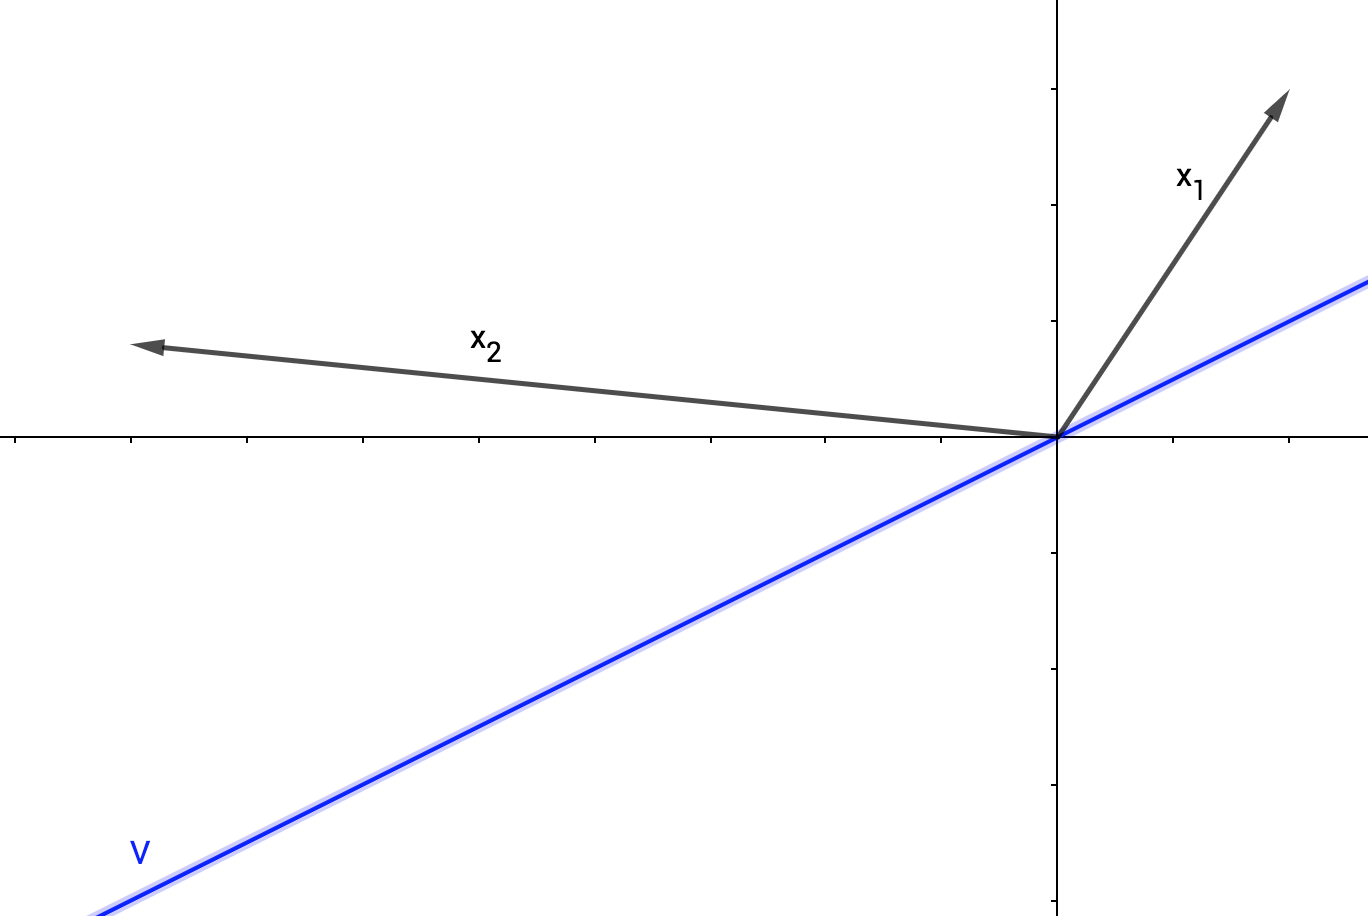
\includegraphics[width=0.7\linewidth]{svd-pic-01}
	\caption{}
	\label{fig:svd-pic-01}
\end{figure}

\noindent If we want to minimize the sum of the squares of the perpendicular distances from the points in $X$ to the subspace $V$, then we will need a basis for $V$. Let's call $\{\mathbf{v}_1\}$ an orthonormal basis for (the yet non-optimal subspace) $V$.\\\leavevmode\\
\begin{figure}
	\centering
	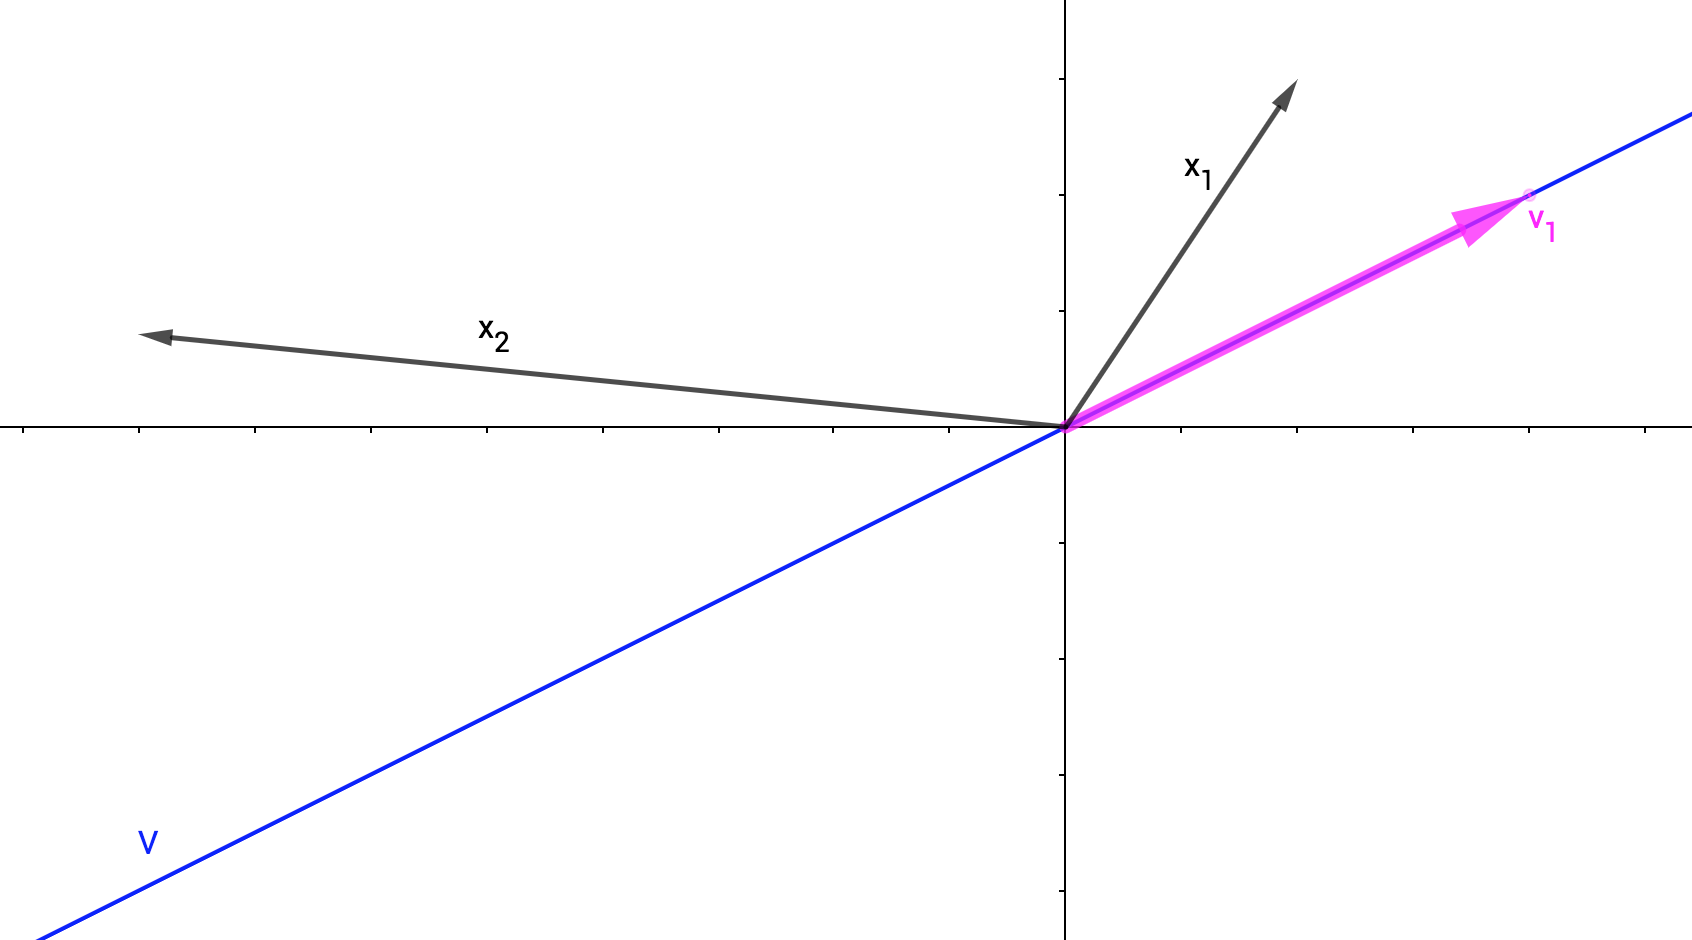
\includegraphics[width=0.7\linewidth]{svd-pic-02}
	\caption{}
	\label{fig:svd-pic-02}
\end{figure}

\noindent And now we want to see the projections of $X$ onto $V$:\\\leavevmode\\
\begin{figure}
	\centering
	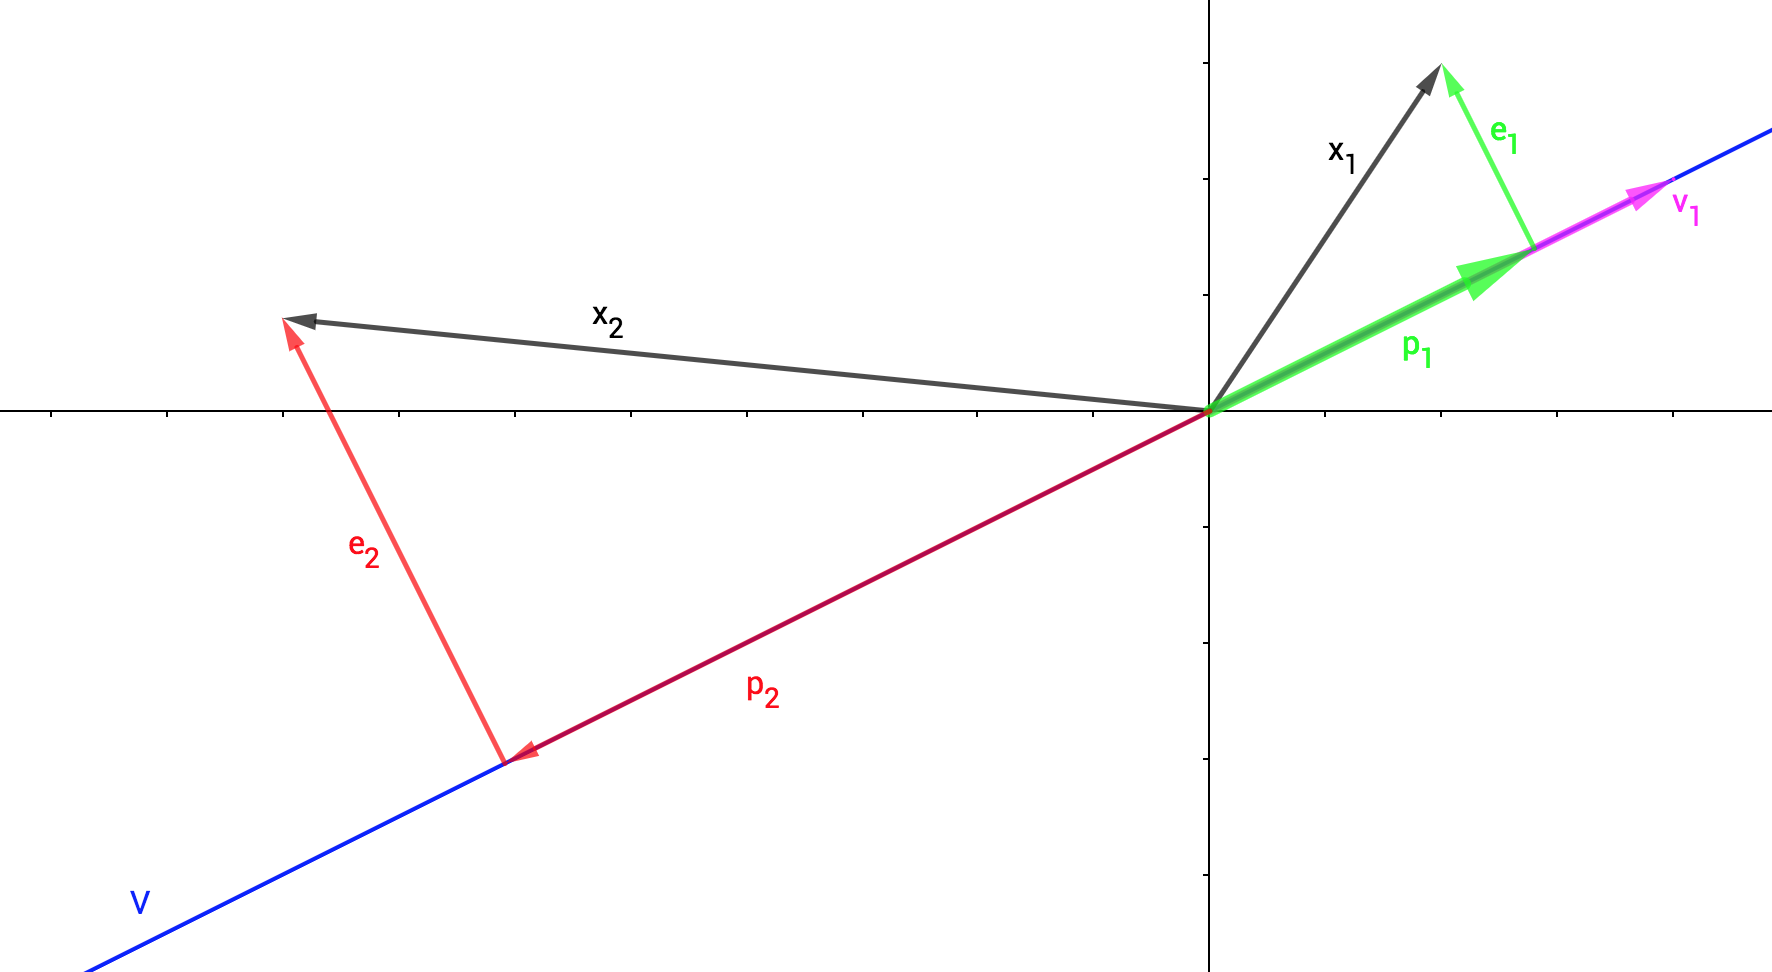
\includegraphics[width=0.7\linewidth]{svd-pic-03}
	\caption{}
	\label{fig:svd-pic-03}
\end{figure}

\noindent$\mathbf{p}_1$ is the projection of $\mathbf{x_1}$ onto $\mathbf{v_1}$ and $\mathbf{p_2}$ is the projection of $\mathbf{x_2}$ onto $\mathbf{v_1}$. $\mathbf{e_1}=\mathbf{x_1}-\mathbf{p_1}$ is the error from the projection of $\mathbf{x_1}$ onto $\mathbf{v_1}$ and $\mathbf{e_2}=\mathbf{x_2}-\mathbf{p_2}$ is the error from the projection of $\mathbf{x_2}$ onto $\mathbf{v_1}$. Recall that, for a given $\mathbf{v_1}$, the error $\mathbf{e_i}$ is minimized when we put $\mathbf{p_i} =\frac{\mathbf{v_1}^T\mathbf{x_i}} {\mathbf{v_1}^T\mathbf{v_1}}\mathbf{v_1}$. It is easy to see and compute that $\mathbf{e_1}$ and $\mathbf{e_2}$ are perpendicular to $\mathbf{v_1}$:
\[
\mathbf{e_i}\cdot\mathbf{v_1}
=
\mathbf{x_i}^T\mathbf{v_1}-\mathbf{p_i}^T\mathbf{v_1}
=
\mathbf{x_i}^T\mathbf{v_1}
-
\Big(\frac{\mathbf{v_1}^T\mathbf{x_i}}{\mathbf{v_1}^T\mathbf{v_1}}\mathbf{v_1}\Big)^T \mathbf{v_1}
\]
\[
=
\mathbf{x_i}^T\mathbf{v_1}
-
\Big(\frac{\mathbf{x_i}^T\mathbf{v_1}}{\mathbf{v_1}^T\mathbf{v_1}}\mathbf{v_1}^T\Big) \mathbf{v_1}
=\mathbf{x_i}^T\mathbf{v_1}-\mathbf{x_i}^T\mathbf{v_1}=0
\]
Similarly, $\mathbf{e_i}$ is perpendicular to $\mathbf{p_i}$:
\[
\mathbf{e_i}\cdot\mathbf{p_i}
=
\mathbf{x_i}^T\mathbf{p_i}-\mathbf{p_i}^T\mathbf{p_i}
=
\mathbf{x_i}^T\mathbf{p_i}
-
\Big(\frac{\mathbf{v_1}^T\mathbf{x_i}}{\mathbf{v_1}^T\mathbf{v_1}}\mathbf{v_1}\Big)^T \mathbf{p_i}
\]
\[
=
\mathbf{x_i}^T\mathbf{p_i}
-
\Big(\frac{\mathbf{x_i}^T\mathbf{v_1}}{\mathbf{v_1}^T\mathbf{v_1}}\mathbf{v_1}^T\Big) \mathbf{p_i}
=
\mathbf{x_i}^T\mathbf{p_i}
-
\frac{\mathbf{x_i}^T\mathbf{v_1}}{\norm{\mathbf{v_1}}^2}\mathbf{p_i}^T \mathbf{v_1}
\]
\[
=
\mathbf{x_i}^T\mathbf{p_i}
-
\mathbf{x_i}^T\mathbf{v_1}\mathbf{p_i}^T \mathbf{v_1}
=
\mathbf{x_i}^T\mathbf{p_i}
-
\mathbf{x_i}^T\mathbf{p_i}\mathbf{v_1}^T \mathbf{v_1}
=
\mathbf{x_i}^T\mathbf{p_i}
-
\mathbf{x_i}^T\mathbf{p_i}
=0
\]
Notice that
\[
0=
\mathbf{e_i}\cdot\mathbf{p_i}
=
\mathbf{x_i}^T\mathbf{p_i}-\mathbf{p_i}^T\mathbf{p_i}
=
\mathbf{p_i}^T\mathbf{x_i}-\mathbf{p_i}^T\mathbf{p_i}
\]
So that
\[
\mathbf{x_i}^T\mathbf{p_i}
=
\mathbf{p_i}^T\mathbf{p_i}
~~\text{and}~~
\mathbf{p_i}^T\mathbf{x_i}
=
\mathbf{p_i}^T\mathbf{p_i}
\]
Hence, for a given $\mathbf{v_1}$, we have:
\[
\norm{\mathbf{e_i}}^2+\norm{\mathbf{p_i}}^2
=
\mathbf{e_i}^T\mathbf{e_i}+\mathbf{p_i}^T\mathbf{p_i}
=
(\mathbf{x_i}-\mathbf{p_i})^T(\mathbf{x_i}-\mathbf{p_i})+\mathbf{p_i}^T\mathbf{p_i}
\]
\[
=
(\mathbf{x_i}^T-\mathbf{p_i}^T)(\mathbf{x_i}-\mathbf{p_i})+\mathbf{p_i}^T\mathbf{p_i}
=\mathbf{x_i}^T\mathbf{x_i}-\mathbf{x_i}^T\mathbf{p_i}-\mathbf{p_i}^T\mathbf{x_i} +\mathbf{p_i}^T\mathbf{p_i}+\mathbf{p_i}^T\mathbf{p_i}
=\norm{\mathbf{x_i}}^2
\]
Succintly, for a given $\mathbf{v_1}$, we have the Pythagorean Theorem:
\[
\norm{\mathbf{e_i}}^2+\norm{\mathbf{p_i}}^2
=\norm{\mathbf{x_i}}^2
\]
Now remember that we haven't yet selected the "best-fit" subspace V nor its basis $\{\mathbf{v_1}\}$. The objective is to find the "optimal" 1-dimensional V such that we minimize the sum of the squares of the perpendicular distances from the points in X to any 1-dimensional subspace. In our simple pictures, the sum of the squares of the perpendicular distances is $\norm{\mathbf{e_1}}^2+\norm{\mathbf{e_2}}^2$:
\[
\norm{\mathbf{e_1}}^2+\norm{\mathbf{e_2}}^2
=
\norm{\mathbf{x_1}}^2+\norm{\mathbf{x_2}}^2
-
\norm{\mathbf{p_1}}^2-\norm{\mathbf{p_2}}^2
\]
So how can we choose V and its basis $\{\mathbf{v_1}\}$ so as to minimize $\norm{\mathbf{e_1}}^2+\norm{\mathbf{e_2}}^2$? Well $\mathbf{x_1}$ and $\mathbf{x_2}$ are given and thus fixed. But $\mathbf{p_1} \equiv\frac{\mathbf{v_1}^T\mathbf{x_1}} {\mathbf{v_1}^T\mathbf{v_1}}\mathbf{v_1}$ and $\mathbf{p_2} \equiv\frac{\mathbf{v_1}^T\mathbf{x_2}} {\mathbf{v_1}^T\mathbf{v_1}}\mathbf{v_1}$ are dependent on $\mathbf{v_1}$, when we select $\mathbf{p_1}$ and $\mathbf{p_2}$ "correctly". Hence we can minimize the sum of the squares of the perpendicular distances by choosing $\mathbf{v_1}$ to maximize $\norm{\mathbf{p_1}}^2+\norm{\mathbf{p_2}}^2$. More generally, we can minimize the sum of the squares of the perpendicular distances between $X$ and $V$ by maximizing the sum of the squared lengths of the projections of $X$ onto $V$. That is, we have converted our original minimization problem into a maximization problem:
\[
\mathbf{v_1}
=
\text{arg max}_
{\mathbf{v}:\norm{\mathbf{v}}=1}\Big(\norm{\mathbf{p_1}}^2+\norm{\mathbf{p_2}}^2\Big)
=
\text{arg max}_
{\mathbf{v}:\norm{\mathbf{v}}=1}\Big(\sum_{i=1}^{2}\norm{\mathbf{p_i}}^2\Big)
\]
\[
=
\text{arg max}_
{\mathbf{v}:\norm{\mathbf{v}}=1}\Big(\sum_{i=1}^{2}\norm{\frac{\mathbf{v}^T\mathbf{x_i}} {\mathbf{v}^T\mathbf{v}}\mathbf{v}}^2\Big)
=
\text{arg max}
_{\mathbf{v}:\norm{\mathbf{v}}=1}\Big(\sum_{i=1}^{2}\norm{\frac{\mathbf{v}^T\mathbf{x_i}} {1}\mathbf{v}}^2\Big)
\]
\[
=
\text{arg max}
_{\mathbf{v}:\norm{\mathbf{v}}=1}\Big(\sum_{i=1}^{2}\norm{(\mathbf{v}^T\mathbf{x_i})\mathbf{v}}^2\Big)
=
\text{arg max}
_{\mathbf{v}:\norm{\mathbf{v}}=1}\Big(\sum_{i=1}^{2}(\mathbf{v}^T\mathbf{x_i})^2\norm{\mathbf{v}}^2\Big)
\]
\[
=
\text{arg max}
_{\mathbf{v}:\norm{\mathbf{v}}=1}\sum_{i=1}^{2}(\mathbf{v}\cdot\mathbf{x_i})^2
\]
But we can write this more compactly by putting the $\mathbf{x_i}$'s into the rows of a matrix, call it $A$:
\[
A=
\begin{bmatrix*}[c]
\mathbf{x_1}^T\\ \mathbf{x_2}^T
\end{bmatrix*}
=
\begin{bmatrix*}[c]
x_{1,1}&x_{1,2}\\
x_{2,1}&x_{2,2}
\end{bmatrix*}
\]
So that
\[
A\mathbf{v}=
\begin{bmatrix*}[c]
x_{1,1}&x_{1,2}\\
x_{2,1}&x_{2,2}
\end{bmatrix*}
\begin{bmatrix*}[c]
v_1\\v_2
\end{bmatrix*}
=
\begin{bmatrix*}[c]
\mathbf{x_1}\cdot\mathbf{v}\\\mathbf{x_2}\cdot\mathbf{v}
\end{bmatrix*}
\]
And
\[
\norm{A\mathbf{v}}^2=
(\mathbf{x_1}\cdot\mathbf{v})^2
+(\mathbf{x_2}\cdot\mathbf{v})^2
\]
And
\[
\mathbf{v_1}=\text{arg max}
_{\mathbf{v}:\norm{\mathbf{v}}=1}\sum_{i=1}^{2}(\mathbf{x_i}\cdot\mathbf{v})^2
=
\text{arg max}_{\mathbf{v}:\norm{\mathbf{v}}=1}\norm{A\mathbf{v}}^2
\]
\[
=
\text{arg max}_{\mathbf{v}:\norm{\mathbf{v}}=1}\norm{A\mathbf{v}}
\]
The last equation follows from the fact the squaring function is a monotonically increasing function.\\\leavevmode\\

\noindent Now let's take this up a notch. Suppose $X=\{\mathbf{x_1},\mathbf{x_2}, \mathbf{x_3}\}$ with $\mathbf{x_i}\in\mathbb{R}^n$. We want to find the plane $V$ in $\mathbb{R}^n$ that minimizes the sum of the squares of the perpendicular distances. That is, the objective is to find an orthonormal basis $\{\mathbf{v_1},\mathbf{v_2}\}$ with $\mathbf{v_i}\in\mathbb{R}^n$ such that we minimize the sum of the squares of the perpendicular distances between $\{\mathbf{x_1},\mathbf{x_2}, \mathbf{x_3}\}$ and $\{\mathbf{v_1}, \mathbf{v_2}\}$.\\\leavevmode\\


\noindent Or even more generally, let $X=\{\mathbf{x_1},...,\mathbf{x_m}\}$ with $\mathbf{x_i}\in\mathbb{R}^n$. The objective is to find some $k$-dimensional subspace of $\mathbb{R}^n$, call it $V$, with orthonormal basis $\{\mathbf{v_1},...,\mathbf{v_k}\}$ such that we minimize the sum of the squares of the perpendicular distances between $\{\mathbf{x_1},...,\mathbf{x_m}\}$ and $\{\mathbf{v_1},...,\mathbf{v_k}\}$. Equivalently, the objective is to find some $k$-dimensional subspace $V\subset\mathbb{R}^n$ with orthonormal basis $\{\mathbf{v_1},...,\mathbf{v_k}\}$ such that we maximize the sum of the squared lengths of the projections of $\{\mathbf{x_1},...,\mathbf{x_m}\}$ onto $\{\mathbf{v_1},...,\mathbf{v_k}\}$.\\\leavevmode\\

\noindent Well just how are we supposed to do that? Maybe "one at a time"? But we must remember to select orthogonal $\mathbf{v_i}$'s:
\[
\mathbf{v_1}
=
\text{arg max}_{\mathbf{v}:\norm{\mathbf{v}}=1}\norm{A\mathbf{v}}
\]
\[
\mathbf{v_2}
=
\text{arg max}_{\mathbf{v}\perp\mathbf{v_1},\norm{\mathbf{v}}=1}\norm{A\mathbf{v}}
\]
For $\mathbf{v_2}$, you see that I added a second condition to the arg max function: $\mathbf{v}\perp\mathbf{v_1}$. So this will get us orthonormal vectors. But will it minimize the sum of the squares of the perpendicular distances between $\{\mathbf{x_1},\mathbf{x_2}, \mathbf{x_3}\}$ and $\{\mathbf{v_1}, \mathbf{v_2}\}$?\\\leavevmode\\

\noindent Before we answer that most important question, let's officially recognize a few things that you have probably noticed. By taking this "one at a time" approach, we are selecting the right singular vectors, the $\mathbf{v_i}$'s. We are also selecting the singular values and left singular vectors:

\[
\sigma_{1}\equiv\text{max}_{\mathbf{v}:\norm{\mathbf{v}}=1}\norm{A\mathbf{v}}
\]
\[
\sigma_{i}\equiv\text{max}_{\mathbf{v}\perp\mathbf{v_1},...,\mathbf{v}\perp\mathbf{v_{i-1}},\norm{\mathbf{v}}=1}\norm{A\mathbf{v}}
\]
\[
\mathbf{u_i}\equiv\frac{A\mathbf{v_i}}{\sigma_{i}}
\]
It is clear that the singular values are monotonically decreasing: $\sigma_{1}\geq\sigma_{2}\geq...\geq\sigma_{k-1}\geq\sigma_{k}$. This follows directly from our definition for each $\sigma_{i}$. Notice that we specify $\norm{A\mathbf{v}}$ (without the square) for the defintion of $\sigma_{1}$ and $\sigma_{i}$, rather than $\norm{A\mathbf{v}}^2$. For the definition of $\mathbf{v_1}$ and $\mathbf{v_i}$, we can use $\norm{A\mathbf{v}}$ and $\norm{A\mathbf{v}}^2$ interchangeably. The monotonicity of the squaring function guarantees that the same $\mathbf{v_i}$ will satisfy both. But for the definition of the singular value $\sigma_{i}$, we specifically want $\norm{A\mathbf{v}}$, without the square. \\\leavevmode\\

\noindent We these definitions, we can actually prove that our "one at a time" approach is equivalent to the "all at once" approach! Let's do that. If you wish to skip this and continue with the "one at a time approach", \hyperlink{btoaata}{\color{blue}{\text{click here}}}. First we define $r(\mathbf{x})=\frac{\mathbf{x}^TS\mathbf{x}}{\mathbf{x}^T\mathbf{x}}$ for a symmetric matrix $S$. This is called the Rayleigh Quotient and it comes in quite handy:\\\leavevmode\\

\noindent{\Large\textbf{Lemma 4: Eigenvectors \& The Rayleigh Quotient}}\\\leavevmode\\
\noindent Suppose $S$ is a symmtric matrix and let $r(\mathbf{x})=\frac{\mathbf{x}^TS\mathbf{x}}{\mathbf{x}^T\mathbf{x}}$. Then $\mathbf{x}\neq\mathbf{0}$ solves $\mathbf{0}=\nabla r(\mathbf{x})$ if and only if $\mathbf{x}$ is an eigenvector of $S$ with eigenvalue $r(\mathbf{x}$).\\\leavevmode\\

\noindent \textbf{Proof}\\
\noindent First we compute the partials:
\[
\frac{\partial r(\mathbf{x})}{\partial x_j}
=
\frac{\frac{\partial}{\partial x_j} \Big(\mathbf{x}^TS\mathbf{x}\Big)}{\mathbf{x}^T\mathbf{x}}
-
\frac{\Big(\mathbf{x}^TS\mathbf{x}\Big)\frac{\partial}{\partial x_j}\Big(\mathbf{x}^T\mathbf{x}\Big)}{(\mathbf{x}^T\mathbf{x})^2}
\]
\[
=
\frac{2(S\mathbf{x})_j}{\mathbf{x}^T\mathbf{x}}
-
\frac{(\mathbf{x}^TS\mathbf{x})2x_j}{(\mathbf{x}^T\mathbf{x})^2}
\]
\[
=
\frac{2}{\mathbf{x}^T\mathbf{x}}
(S\mathbf{x}-r(\mathbf{x})\mathbf{x})_j
\]
So our gradient is $\nabla r(\mathbf{x})=\frac{2}{\mathbf{x}^T\mathbf{x}}(S\mathbf{x}-r(\mathbf{x})\mathbf{x})$ and we find that
\[
\mathbf{0}=
\nabla r(\mathbf{x})=\frac{2}{\mathbf{x}^T\mathbf{x}}(S\mathbf{x}-r(\mathbf{x})\mathbf{x})
\]
\[
\iff
\mathbf{0}
=
S\mathbf{x}-r(\mathbf{x})\mathbf{x}
\]
\[
\iff
S\mathbf{x}=r(\mathbf{x})\mathbf{x}
\]
\qedsymbol\\\leavevmode\\

\noindent This lemma tells us is that the stationary points of $r(\mathbf{x})=\frac{\mathbf{x}^TS\mathbf{x}}{\mathbf{x}^T\mathbf{x}}$ are eigenvectors for $S$ with eigenvalues equal to $r(\mathbf{x})$ at those points. Hence we can set $S=A^TA$ and get the largest eigenvalue by computing $\lambda_1=\text{max}_\mathbf{x}r(\mathbf{x})=\text{max}_\mathbf{x}\frac{\mathbf{x}^TA^TA\mathbf{x}}{\mathbf{x}^T\mathbf{x}}=\text{max}_\mathbf{x}\frac{\norm{A\mathbf{x}}^2}{\norm{\mathbf{x}}^2}$ and

\[
\lambda_1=
\text{max}_{\mathbf{v}:\norm{\mathbf{v}}=1}\norm{A\mathbf{v}}^2=\sigma_{1}^2
\]
\[
\mathbf{v_1}=
\text{arg max}_{\mathbf{v}:\norm{\mathbf{v}}=1}\norm{A\mathbf{v}}^2
\]
So $\lambda_1=\sigma_{1}^2$ is the largest eigenvalue of $A^TA$ with corresponding eigenvector $\mathbf{v_1}$. Of course these are the same values we computed above to maximize the sum of the squared lengths of the projections of $X$ onto $V$. Similarly, lemma 4 says that
\[
\lambda_i=
\text{max}_{\mathbf{v}\in\text{span}(\mathbf{v_1},...,\mathbf{v_{i-1}})^\perp,\norm{\mathbf{v}}=1}\norm{A\mathbf{v}}^2=\sigma_{i}^2
\]
\[
\mathbf{v_i}=
\text{arg max}_{\mathbf{v}\in\text{span}(\mathbf{v_1},...,\mathbf{v_{i-1}})^\perp,\norm{\mathbf{v}}=1}\norm{A\mathbf{v}}^2
\]
\noindent is the i$^{\text{th}}$ largest eigenpair for $A^TA$ since $\mathbf{v_i}$ is a stationary point of $r(\mathbf{x})$.\\\leavevmode\\

\noindent So how does this show that the "all at once" approach is equivalent to this "one at a time" approach? Well, in the first few lines of that proof, we picked the right singular vectors to be orthonormal eigenvectors of $A^TA$. And we defined the singulars values to be the square roots of the corresponding eigenvalues. Everything else in the proof follows from that. But now we have shown than the $\mathbf{v_i}$'s and $\sigma_{i}^2$'s defined to maximize the sum of the squared lengths of the projections of $X$ onto $V$ are in fact orthonormal eigenpairs for $A^TA$. Hence equivalency.\\\leavevmode\\

\noindent Incidentally, this leads directly to another proof of the Spectral Theorem. By iteratively computing the $\lambda_i$'s and orthonormal $\mathbf{v_i}$'s for any given symmetric matrix $S$ using the max, argmax of the Rayleigh Quotient, we are also computing $S=\sum_{i=1}^n\lambda_i\mathbf{v_i}\mathbf{v_i}^T=V\Lambda V^T$.\\\leavevmode\\

\noindent \hypertarget{btoaata}{\text{OK, back to our "one at a time" approach.}} Now you might be asking, can we do this iterative step $n$ times? Well, as long as $\norm{A\mathbf{v}}>0$, then you will have $n$ positive singular values: $\sigma_{i}>0$ for $i=1,...,n$. And you will have an orthonormal basis $\{\mathbf{v_i},...,\mathbf{v_n}\}$ for $\mathbb{R}^n$. As we proved in the "all at once" proof, $A$ has rank $n$.\\\leavevmode\\

\noindent But what happens when $\sigma_{k}>0$ but $\sigma_{k+1}=0$ for some $k<n$? This must mean that the rank of $A$ is $k$. Let's see why that must be the case. Here's what we have: For any $j>k$, any $\mathbf{v_{j}}$ satisfying $\mathbf{v_{j}}\perp \mathbf{v_i}$ for all $i=1,...,k$ must also satisfy $\norm{A\mathbf{v_{j}}}= \sigma_{j}=0$. Such $\mathbf{v_{j}}$'s must also satisfy $A\mathbf{v_{j}}=\mathbf{0}$. That is, the only remaining $\mathbf{v_{j}}$'s that are orthogonal to all $\{\mathbf{v_1},...,\mathbf{v_k}\}$ must be in the nullspace of $A$. Since the dimension of $\mathbb{R}^n$ is $n$, surely we can select $n-k$ such $\mathbf{v_{j}}$'s. Said another way, we can extend $\{\mathbf{v_1},...,\mathbf{v_k}\}$ to an orthonormal basis for $\mathbb{R}^n$ but only with $\mathbf{v_{j}}$'s that are in the nullspace of $A$. Hence the nullspace of $A$ has dimension $n-k$ and hence $A$ has rank $k$.\\\leavevmode\\

\noindent In this case where the rank of $A$ is $k$ for $k<n$, you have $k$ positive singular values: $\sigma_{i}>0$ for $i=1,...,k$. And you have $k$ right singular vectors $\{\mathbf{v_i}:i=1,...,k\}$. Then you can put $\sigma_{i}=0$ for $i>k$ to get $n$ nonnegative singular values: $\sigma_{1}\geq\sigma_{2}\geq ...\geq\sigma_{n-1}\geq\sigma_{n}=0$. And you can extend $\{\mathbf{v_1},...,\mathbf{v_k}\}$ with any orthonormal basis $\{\mathbf{v_{k+1}},...,\mathbf{v_n}\}$ for the nullspace of $A$ to get a full set of right singular vectors $\{\mathbf{v_1},...,\mathbf{v_k}, \mathbf{v_{k+1}},...,\mathbf{v_n}\}$.\\\leavevmode\\

\noindent One last piece of terminology: We will say a $k$-dimensional subspace $V$ is \textbf{best-fit} or \textbf{optimal} for a matrix $A$ if it minimizes the sum of the squares of the perpendicular distances between the rows of $A$ and all $k$-dimensional subspaces. Equivalently, a subspace $V$ is \textbf{best-fit} or \textbf{optimal} for $A$ if it maximizes the sum of the squared lengths of the projections of the rows of $A$ onto all $k$-dimensional subspaces.\\\leavevmode\\

\noindent OK, finally, let's state and prove the "alternate" form of SVD:\\\leavevmode\\

\noindent{\Large\textbf{Theorem: Alternate Singular Value Decomposition}}\\\leavevmode\\
\noindent Let $A_{m~\times~n}=\begin{bmatrix*}[c]
\mathbf{x_1}^T\\\vdots\\\mathbf{x_m}^T
\end{bmatrix*}$, $\mathbf{x_i}\in\mathbb{R}^n$, where the rank of $A$ is $r$. Let $\{\mathbf{v_1},...,\mathbf{v_r}\}$ be its right singular vectors and let $\{\sigma_{1},...,\sigma_{r}\}$ be its singular values:

\[
\mathbf{v_i},~\sigma_{i}\equiv\text{argmax, max}_{\mathbf{v}\perp\mathbf{v_1},...,\mathbf{v}\perp\mathbf{v_{i-1}},\norm{\mathbf{v}}=1}\norm{A\mathbf{v}}
\]
 For any $k\leq r$, $V_k\equiv$ Span$\{\mathbf{v_1},...,\mathbf{v_k}\}$ is the best-fit $k$-dimensional vector subspace for $A$.\\\leavevmode\\

\noindent{\Large\textbf{SVD Proof: One At A Time}}\\\leavevmode\\

\noindent For $k=1$, we have already shown that this reduces to a least squares fitting problem for which $\mathbf{v_1}$ is the solution. For $k = 2$, let $W$ be a best-fit 2-dimensional subspace for $A$. For any basis $\mathbf{w_1}$, $\mathbf{w_2}$ of $W$, $\norm{A\mathbf{w_1}}+\norm{A\mathbf{w_2}}$ is the sum of
squared lengths of the projections of the rows of $A$ onto $W$. Now, choose a basis $\mathbf{w_1}$, $\mathbf{w_2}$ of $W$ so that $\mathbf{w_2}$ is perpendicular to $\mathbf{v_1}$. If $\mathbf{v_1}$ is perpendicular to $W$, any unit vector in $W$ will do as $\mathbf{w_2}$. If not, choose $\mathbf{w_2}$ to be the unit vector in $W$ perpendicular to the projection of $\mathbf{v_1}$ onto $W$. Since $\mathbf{v_1}$ was chosen to maximize $\norm{A\mathbf{v}}^2$, it follows that $\norm{A\mathbf{w_1}}^2\leq\norm{A\mathbf{v_1}}^2$. Since $\mathbf{v_2}$ was chosen to maximize $\norm{A\mathbf{v}}^2$ over all $\mathbf{v}$ perpendicular to $\mathbf{v_1}$, $\norm{A\mathbf{w_2}}^2\leq\norm{A\mathbf{v_2}}^2$. Hence
\[
\norm{A\mathbf{w_1}}^2+\norm{A\mathbf{w_2}}^2
\leq
\norm{A\mathbf{v_1}}^2+\norm{A\mathbf{v_2}}^2
\]
and $V_2$ is at least as good as $W$ and so is a best-fit 2-dimensional subspace.\\\leavevmode\\

\noindent For general $k$, proceed by induction. By the induction hypothesis, $V_{k-1}$ is a best-fit $k-1$ dimensional subspace. Suppose $W$ is a best-fit $k$-dimensional subspace. Choose a basis $\mathbf{w_1}$, $\mathbf{w_2}$,..., $\mathbf{w_k}$ of $W$ so that $\mathbf{w_k}$ is perpendicular to $\mathbf{v_1}$, $\mathbf{v_2}$,..., $\mathbf{v_{k-1}}$. Then
\[
\norm{A\mathbf{w_1}}^2+\norm{A\mathbf{w_2}}^2+...+\norm{A\mathbf{w_k}}^2
\leq
\norm{A\mathbf{v_1}}^2+\norm{A\mathbf{v_2}}^2+...+\norm{A\mathbf{v_{k-1}}}^2+\norm{A\mathbf{w_k}}^2
\]
since $V_{k-1}$ is an optimal $k-1$ dimensional subspace. Since $\mathbf{w_k}$ is perpendicular to
$\mathbf{v_1}$, $\mathbf{v_2}$,..., $\mathbf{v_{k-1}}$, by the definition of $\mathbf{v_k}$, $\norm{A\mathbf{w_k}}^2\leq\norm{A\mathbf{v_k}}^2$. Thus
\[
\norm{A\mathbf{w_1}}^2+\norm{A\mathbf{w_2}}^2+...+\norm{A\mathbf{w_{k-1}}}^2+\norm{A\mathbf{w_k}}^2
\leq
\norm{A\mathbf{v_1}}^2+\norm{A\mathbf{v_2}}^2+...+\norm{A\mathbf{v_{k-1}}}^2+\norm{A\mathbf{v_k}}^2
\]
proving that $V_k$ is at least as good as $W$ and hence is optimal.\quad\qedsymbol\\\leavevmode\\

\noindent Now we would like to find a reasonably efficient algorithm for computing the singular vectors and singular values.\\\leavevmode\\

\noindent{\Large\textbf{The Power Method}}\\\leavevmode\\
\noindent For (just about) any $\mathbf{x}\in\mathbb{R}^n$ and any $m~\times~n$ matrix $A$:
\[
\lim_{s\rightarrow\infty}\frac{(A^TA)^s\mathbf{x}}{\norm{(A^TA)^s\mathbf{x}}}
=\mathbf{v_1}~~~~\text{if and only if }\sigma_{1}>\sigma_{2}
\]
where $\mathbf{v_1}$ is the first right singular vector and $\sigma_{1}$ and $\sigma_{2}$ are the first and second singular values of $A$.\\\leavevmode\\
\noindent{\textbf{Proof}}\\\leavevmode\\

\noindent First we need to find a convenient formula for $(A^TA)^s$. Suppose $A$ has rank $r$ and orthonormal right singular vectors $\mathbf{v_1},...,\mathbf{v_n}$. Then 
\[
(A^TA)^2=\Big(\sum_{i=1}^{r}\sigma_i^2\mathbf{v_i}\mathbf{v_i}^T\Big)^2
=
\Big(\sum_{i=1}^{r}\sigma_i^2\mathbf{v_i}\mathbf{v_i}^T\Big)
\Big(\sum_{j=1}^{r}\sigma_j^2\mathbf{v_j}\mathbf{v_j}^T\Big)
\]
\[
=
\sum_{i,j=1}^{r}\sigma_i^2\sigma_j^2\mathbf{v_i}\mathbf{v_i}^T\mathbf{v_j}\mathbf{v_j}^T
=
\sum_{i=1}^{r}\sigma_i^4\mathbf{v_i}\mathbf{v_i}^T
\]
Inductively, we find that
\[
(A^TA)^s=
\sum_{i=1}^{r}\sigma_i^{2s}\mathbf{v_i}\mathbf{v_i}^T
\]
\noindent Aside: The outer product is more convenient here but we also could have found
\[
A^TA=(U\Sigma V^T)^T(U\Sigma V^T)=V\Sigma^TU^TU\Sigma V^T=V\Sigma^2V^T
\]
The last equation follows from the orthonormality of $U$ so that $U^TU=I$. Also $\Sigma$ is diagonal and hence symmetric: $\Sigma^T=\Sigma$. Similarly, we can compute
\[
(A^TA)^2=V\Sigma^2V^TV\Sigma^2V^T=V\Sigma^4V^T
\]
And inductively find
\[
(A^TA)^s=V\Sigma^{2s}V^T
\]
\noindent Anyway, back to the proof: since $\{\mathbf{v_1},...,\mathbf{v_n}\}$ is an orthonormal basis for $\mathbb{R}^n$, there exists scalars $c_1,...,c_n$ such that $\mathbf{x}=\sum_{i=1}^nc_i\mathbf{v_i}$. And we can compute
\[
A^TA\mathbf{x}=
\Big(\sum_{i=1}^{n}\sigma_i^2\mathbf{v_i}\mathbf{v_i}^T\Big)\Big(\sum_{j=1}^nc_j\mathbf{v_j}\Big)
=
\sum_{i,j=1}^{n}\sigma_i^2\mathbf{v_i}\mathbf{v_i}^Tc_j\mathbf{v_j}
=
\sum_{i=1}^nc_i\sigma_{i}^2\mathbf{v_i}
=
\sum_{i=1}^rc_i\sigma_{i}^2\mathbf{v_i}
\]
Similarly, using our handy formula for $(A^TA)^s$, we find that
\[
(A^TA)^s\mathbf{x}=
\sum_{i=1}^rc_i\sigma_{i}^{2s}\mathbf{v_i}
\]
We also need a handy formula for $\norm{(A^TA)^s\mathbf{x}}$:
\[
\norm{(A^TA)^s\mathbf{x}}^2=
((A^TA)^s\mathbf{x})^T((A^TA)^s\mathbf{x})
=
\Big(\sum_{i=1}^rc_i\sigma_{i}^{2s}\mathbf{v_i}\Big)^T\Big(\sum_{j=1}^rc_j\sigma_{j}^{2s}\mathbf{v_j}\Big)
\]
\[
=
\Big(\sum_{i=1}^rc_i\sigma_{i}^{2s}\mathbf{v_i}^T\Big)\Big(\sum_{j=1}^rc_j\sigma_{j}^{2s}\mathbf{v_j}\Big)
=
\sum_{i,j=1}^rc_ic_j\sigma_{i}^{2s}\sigma_{j}^{2s}\mathbf{v_i}^T\mathbf{v_j}
=\sum_{i=1}^rc_i^2\sigma_{i}^{4s}
\]
So we have a tractable formula for $\frac{(A^TA)^s\mathbf{x}}{\norm{(A^TA)^s\mathbf{x}}}$ as well:
\[
\frac{(A^TA)^s\mathbf{x}}{\norm{(A^TA)^s\mathbf{x}}}
=
\frac{1}{\norm{(A^TA)^s\mathbf{x}}}\sum_{i=1}^rc_i\sigma_{i}^{2s}\mathbf{v_i}
=
\frac{1}{\sqrt{\sum_{j=1}^rc_j^2\sigma_{j}^{4s}}}\sum_{i=1}^rc_i\sigma_{i}^{2s}\mathbf{v_i}
\]
\[
=
\sum_{i=1}^r\frac{c_i\sigma_{i}^{2s}}{\sqrt{\sum_{j=1}^rc_j^2\sigma_{j}^{4s}}}\mathbf{v_i}
\]
So let's compute $\lim_{s\rightarrow\infty}\frac{c_i\sigma_{i}^{2s}}{\sqrt{\sum_{j=1}^rc_j^2\sigma_{j}^{4s}}}$:
\[\lim_{s\rightarrow\infty}\frac{c_i\sigma_{i}^{2s}}{\sqrt{\sum_{j=1}^rc_j^2\sigma_{j}^{4s}}}
=
\lim_{s\rightarrow\infty}\sqrt{\frac{c_i^2\sigma_{i}^{4s}}{\sum_{j=1}^rc_j^2\sigma_{j}^{4s}}}
=
\sqrt{\lim_{s\rightarrow\infty}\frac{c_i^2\sigma_{i}^{4s}}{\sum_{j=1}^rc_j^2\sigma_{j}^{4s}}}
\]
\[
=
\sqrt{\lim_{s\rightarrow\infty}\frac{1}{1+\frac{1}{c_i^2\sigma_{i}^{4s}}\sum_{j=1,j\ne i}^rc_j^2\sigma_{j}^{4s}}}
=
\sqrt{\lim_{s\rightarrow\infty}\frac{1}{1+\sum_{j=1,j\ne i}^r\frac{c_j^2\sigma_{j}^{4s}}{c_i^2\sigma_{i}^{4s}}}}
\]
\[
=
\sqrt{\lim_{s\rightarrow\infty}\frac{1}{1+\sum_{j=1,j\ne i}^r(\frac{c_j}{c_i})^2(\frac{\sigma_{j}}{\sigma_{i}})^{4s}}}
\]
For $i=1$, we have
\[
\lim_{s\rightarrow\infty}\frac{c_1\sigma_{1}^{2s}}{\sqrt{\sum_{j=1}^rc_j^2\sigma_{j}^{4s}}}
=\begin{cases*}
1&if $\sigma_{1}>\sigma_{2}$\\
\sqrt{\frac{1}{1+(\frac{c_2}{c_1})^2}}&if $\sigma_{1}=\sigma_{2}$
\end{cases*}
\]
Of course we are also assuming that the random vector $\mathbf{x}$ has a nonzero first compotent $c_1\ne0$ (this is the "just about" disclaimer in the theorem statement). For $i=2$, we have
\[
\lim_{s\rightarrow\infty}\frac{c_2\sigma_{2}^{2s}}{\sqrt{\sum_{j=1}^rc_j^2\sigma_{j}^{4s}}}
=\begin{cases*}
0&if $\sigma_{1}>\sigma_{2}$\\
\sqrt{\frac{1}{1+(\frac{c_1}{c_2})^2}}&if $\sigma_{1}=\sigma_{2}$
\end{cases*}
\]
And putting it together:
\[
\lim_{s\rightarrow\infty}\frac{(A^TA)^s\mathbf{x}}{\norm{(A^TA)^s\mathbf{x}}}
=
\lim_{s\rightarrow\infty}\sum_{i=1}^r\frac{c_i\sigma_{i}^{2s}}{\sqrt{\sum_{j=1}^rc_j^2\sigma_{j}^{4s}}}\mathbf{v_i}
=\mathbf{v_1}~~~~\text{so long as }\sigma_{1}>\sigma_{2}
\]
\qedsymbol\\\leavevmode\\
\noindent Of course, once we have numerically computed $\mathbf{v_1}$, we can use the Rayleigh Quotient to get the corresponding eigenvalue of $A^TA$ which is also the square of the singular value of $A$: $\sigma_{1}^2=\lambda_1=r(\mathbf{v_1})=\frac{\mathbf{v_1
}^TA^TA\mathbf{v_1}}{\mathbf{v_1}^T\mathbf{v_1}}=\mathbf{v_1
}^TA^TA\mathbf{v_1}=(A\mathbf{v_1})^TA\mathbf{v_1}=\mathbf{u_1}^T\mathbf{u_1}$. And then we can normalize $\mathbf{u_1}$ to finish off the first pair of singular vectors.\\\leavevmode\\

\noindent  Since we have computed $\sigma_{1}$, $\mathbf{v_1}$, and $\mathbf{u_1}$, we can
repeat this procedure for $A-\sigma_{1}\mathbf{u_1}\mathbf{v_1}^T$. The top singular value and vectors of this matrix are $\sigma_2$, $\mathbf{v_1}$, and $\mathbf{u_2}$. Repeating this procedure $k$ times will get us the top $k$ singular values and vectors and the best-fit $k$-dimensional subspace $V_k=\text{Span}\{\mathbf{v_1,...,\mathbf{v_k}}\}$.\\\leavevmode\\

\noindent So the question becomes, how quickly does $\frac{(A^TA)^s\mathbf{x}}{\norm{(A^TA)^s\mathbf{x}}}$ converge to $\mathbf{v_1}$? Well, the Power Method isn't industrial strength, but it's still pretty good. You can find a \Waynehref{https://en.wikipedia.org/wiki/Power_iteration\#Analysis}{\text{detailed analysis here}} or \Waynehref{http://www.cs.yale.edu/homes/el327/datamining2013aFiles/07_singular_value_decomposition.pdf}{\text{at the end this}}. It turns out that the convergence is geometric with ratio $\frac{\lambda_2}{\lambda_1}$.\\\leavevmode\\

\noindent When we actually code this up, when we're computing an approximation for some $\mathbf{v_i}$, instead of iterating a calculated number of times, we will simply stop iterating when the angle between iteration results is sufficiently small. What does that mean? Let $\mathbf{t_s}=\frac{(A^TA)^s\mathbf{x}}{\norm{(A^TA)^s\mathbf{x}}}$. Then $\mathbf{t_s}$ is a unit vector. So the $cos$ of the angle $\theta_s$ between $\mathbf{t_s}$ and $\mathbf{t_{s-1}}$ can be computed as $cos(\theta_s)=\frac{\mathbf{t_s}\cdot\mathbf{t_{s-1}}}{\norm{\mathbf{t_s}}\norm{\mathbf{t_{s-1}}}}=\mathbf{t_s}\cdot\mathbf{t_{s-1}}$. We know that $\text{lim}_{\theta\rightarrow0}cos(\theta)=1$ and that $cos(\theta)\leq1$ for all $\theta$. At each iteration $s$, we check whether $\mathbf{t_s}\cdot\mathbf{t_{s-1}}>1-\epsilon$ for some arbitrarily small $\epsilon$. When this check is true for some iteration $s$, we have a sufficiently small angle between iteration results and we're not going to get a much better approximation for $\mathbf{v_i}$ than $\mathbf{t_s}$. So we stop.

\end{document}